% Revision draft of 30 October 2026, prepared from review_volatility_models_revised_20261028.tex
% (unchanged) after the manuscript review of 29 October 2026 (agents/review-volatility-models-revision-ijtaf-2026-10-29.md).
% Structural changes: closure proposition (Prop. 2.2), rewritten abstract and contributions, kappa_2 = 0 paragraph,
% per-maturity calibration table and cost statement, references, supplement split (supplement_20261030.tex).
% Generated prose blocks are delimited by "% [AI-DRAFT BEGIN ...]" / "% [AI-DRAFT END]". Outside those blocks the
% 30 Oct pass removed prose semicolons, contrastive "X; it is not Y" pairs and paragraph-final restatements, and
% did not alter any equation, number or citation. Author passes pending: crux sentence of Section 1 (marked CRUX).
% Generated inputs: empirical_bloomberg_20261030/ (empirical section, macros) and calibration_section_20261030/
% (calibration section, macros). Numbers in prose are macros from those files, never typed.
% Equation-review recommendations implemented on 30 October 2026; see repository agents/robust_volatility_review_20261030/implementation/.
% Length cut of 30 October 2026 (round 3, agents/2026-10-30_REVISION_LOG.md): seven figures and one table moved to the
% replication package, the supplement document (supplement_20261030.tex) is kept buildable as package notes and is not submitted.
% Revision pass of 17 November 2026, implementing agents/robust-volatility-models-submission-readiness-2026-11-16.md:
% abstract, definition of robustness in Section 1, new Section 2.4 (closure under affine Girsanov kernels, Prop. 2.3,
% Tables tab:kernel-closure and tab:numeraires), notation table, SABR and literature additions, symbol renames
% (Volterra exponent, diffusion coefficient of Section 6.3, moment order of Table 2, exponent of Appendix A) and spelling.
% New generated text sits in "% [AI-DRAFT BEGIN: ..., 17 Nov 2026]" blocks. "% [AUTHOR: ...]" comments mark author items.
% Four numbered equations were added, so equation numbers differ from the 30 October build (mapping in the report).
% Second pass of 17 November 2026 (report Section 10): Section 5.1 and Table tab:nonmarkov follow revision 2 of the
% Volterra paper, the annuity row of Table tab:numeraires was checked against factor_sv_model.tex, the second author's
% affiliation, per-model half-life macros, bibliographic data and table-cell semicolons were completed. The crux of
% Section 1 and the mechanism sentences before Propositions 2.3 and 4.1 are drafted in "% [AI-DRAFT CRUX ...]" and
% "% [AI-DRAFT MECHANISM ...]" blocks. By the drafting-order rule they remain the author's to rewrite.
\documentclass[11pt,a4paper]{article}
\usepackage[T1]{fontenc}
\usepackage[utf8]{inputenc}
\usepackage{lmodern}
\usepackage{amsmath,amssymb,amsthm}
\usepackage[margin=25mm]{geometry}
\usepackage{booktabs,longtable,array,tabularx}
\usepackage{graphicx}
\usepackage{placeins}
\usepackage{ragged2e}
\usepackage{enumitem}
\usepackage{microtype}
\usepackage{natbib}
\usepackage{xcolor}
\usepackage{hyperref}
\hypersetup{colorlinks=true,linkcolor=blue,citecolor=blue,urlcolor=blue,
 pdftitle={What Is a Robust Stochastic Volatility Model?},
 pdfauthor={Artur Sepp and Parviz Rakhmonov}}
\newtheorem{proposition}{Proposition}[section]
\newtheorem{lemma}[proposition]{Lemma}
\newtheorem{corollary}[proposition]{Corollary}
\theoremstyle{definition}
\newtheorem{definition}[proposition]{Definition}
\newtheorem{assumption}[proposition]{Assumption}
\theoremstyle{remark}
\newtheorem*{remark}{Remark}
\newcommand{\E}{\mathbb{E}}
\newcommand{\PP}{\mathbb{P}}
\newcommand{\QQ}{\mathbb{Q}}
\newcommand{\QS}{\mathbb{Q}^{S}}
\newcommand{\RR}{\mathbb{R}}
\newcommand{\dd}{\,\mathrm{d}}
\newcommand{\ind}{\mathbf{1}}
\DeclareMathOperator{\Var}{Var}
\DeclareMathOperator{\Corr}{Corr}
\DeclareMathOperator{\Cov}{Cov}
\newcolumntype{P}[1]{>{\RaggedRight\arraybackslash}p{#1}}
% Float pages only when at least 75% full (half-page figures sit at the top of text pages instead).
\renewcommand{\floatpagefraction}{.75}
\renewcommand{\topfraction}{.8}
\setlength{\emergencystretch}{2em}
\setlist{itemsep=3pt,topsep=5pt}
% Longtable captions use the full text width (they were set narrower than their tables).
\setlength{\LTcapwidth}{\textwidth}
% Number macros generated by the replication code (see header). Edit the generators, not these files.
% Generated by empirical_bloomberg_20261030/make_empirical_section.py. Do not edit.

\newcommand{\betaPosVIX}{0.0}

\newcommand{\betaPosOVX}{17.0}

\newcommand{\betaPosMOVE}{63.9}

\newcommand{\betaPosGVZ}{53.4}

\newcommand{\betaPosVXTLT}{46.3}

\newcommand{\panelCount}{15}

\newcommand{\panelGigWins}{13}

\newcommand{\panelGigSig}{9}

\newcommand{\panelGigSigNeg}{1}

\newcommand{\scoreVIXsqrtGamma}{0.163}

\newcommand{\scoreVIXsqrtIG}{-0.009}

\newcommand{\igShapeVIX}{8.0}

\newcommand{\igShapeOVX}{8.0}

\newcommand{\commonSessions}{2898}

\newcommand{\betaPosBTCDVOL}{34.8}

\newcommand{\acfBTCDVOL}{0.703}

\newcommand{\scoreBTCDVOLHeston}{0.028}

\newcommand{\scoreBTCDVOLThreeHalf}{0.036}

\newcommand{\betaPosETHDVOL}{30.4}

\newcommand{\acfETHDVOL}{0.600}

\newcommand{\scoreETHDVOLHeston}{0.081}

\newcommand{\scoreETHDVOLThreeHalf}{-0.093}

% Generated by calibration_section_20261030/make_calibration_section.py. Do not edit.
\newcommand{\rmseHestonSPXW}{0.70}
\newcommand{\rmseLogSVSPXW}{0.45}
\newcommand{\insideLogSVSPXW}{20.4}
\newcommand{\insideHestonSPXW}{8.7}
\newcommand{\rmseHestonGLD}{0.48}
\newcommand{\rmseLogSVGLD}{0.34}
\newcommand{\insideLogSVGLD}{73.5}
\newcommand{\insideHestonGLD}{55.9}
\newcommand{\rmseHestonTLT}{0.46}
\newcommand{\rmseLogSVTLT}{0.29}
\newcommand{\insideLogSVTLT}{58.4}
\newcommand{\insideHestonTLT}{37.1}
\newcommand{\rmseHestonTLTpositive}{0.80}
\newcommand{\rmseLogSVTLTpositive}{0.58}
\newcommand{\insideLogSVTLTpositive}{32.3}
\newcommand{\insideHestonTLTpositive}{24.2}
\newcommand{\fitRatioMax}{2,367}
\newcommand{\fitRatioMin}{806}
\newcommand{\halfLifeLogSVMin}{7.4}
\newcommand{\halfLifeLogSVMax}{10.0}
\newcommand{\halfLifeHestonMin}{8.4}
\newcommand{\halfLifeHestonMax}{10.4}
\newcommand{\surfaceCount}{4}
\newcommand{\improvedSlices}{15}
\newcommand{\totalSlices}{16}
\newcommand{\positiveBeta}{1.433}
\newcommand{\positiveKappaTwo}{31.018}
\newcommand{\positiveMargin}{29.585}
\newcommand{\positiveHestonRho}{0.196}

\title{What Is a Robust Stochastic Volatility Model?\\
 \large Measure Changes, Martingality and Cross-Asset Applications}
\author{Artur Sepp\thanks{LGT Bank (Schweiz) AG, Z\"urich. Contact: \href{mailto:artursepp@gmail.com}{artursepp@gmail.com}.}
 \and Parviz Rakhmonov\thanks{Marex, London, United Kingdom. Contact: \href{mailto:parviz.msu@gmail.com}{parviz.msu@gmail.com}.}}
% [AUTHOR: the second author's affiliation and address are those printed in the RDR 2025 and IJTAF 2023 papers. Confirm that they are current.]
% Cover-letter line, removed from the title block on 17 Nov 2026:
% 30 October 2026, revision of the working paper of 27 November 2023 (SSRN 4647027).
\date{24 November 2026}

\begin{document}
\maketitle

\begin{abstract}
% [AI-DRAFT BEGIN: abstract, one sentence per element (context, gap, method, result, implication), rewritten 17 Nov 2026. Numbers are macros. 198 words.]
Stochastic-volatility models are estimated under the physical measure and used under pricing measures and asset-specific numeraires, where several specifications lose the true-martingale property when the return--volatility dependence is positive. Existing treatments mix six requirements, from drift-family closure to numerical reliability, and apply them unevenly across Heston, lognormal and rough specifications. We characterise closure of polynomial volatility drifts under Girsanov kernels affine in volatility, which cover stock and foreign-currency numeraires, quanto adjustments and risk prices, and prove that lognormal volatility with drift $A+B\sigma-C\sigma^2$ and loading $\beta$ on the return noise makes the discounted asset a true martingale on every finite horizon if and only if $C\geq\beta$, boundary cases included. Of seven diffusion specifications only signed Gaussian and quadratic-drift lognormal volatility are closed under all such kernels, a positive observed volatility beta occurs on \betaPosVIX\% to \betaPosGVZ\% of days across \panelCount{} Cboe volatility indices, a generalised inverse Gaussian marginal outscores the Heston marginal out of sample for \panelGigWins{} of them, and the lognormal model lowers Heston's implied-volatility error on four option snapshots, one with positive skew and $\beta=\positiveBeta$, at \fitRatioMin{} to \fitRatioMax{} times the calibration time. A selection guide maps application requirements to admissibility conditions, observation conventions and validation steps.
% [AI-DRAFT END]
\end{abstract}

\noindent\textbf{Keywords:} stochastic volatility, change of numeraire, true martingale, lognormal volatility, Heston model, 3/2 model, rough volatility, option calibration.\\
\textbf{JEL:} C58, G13. \quad \textbf{MSC 2020:} 60H30, 91G20, 91G60.

\section{Introduction}
\label{sec:introduction}

A stochastic-volatility model is used for more than fitting a single option surface. Its parameters may be estimated from historical observations, transferred to a pricing measure, and used for products with different settlement or numeraire conventions. The model must remain well defined throughout that application. This issue is particularly visible when the return--volatility dependence is positive, or changes sign across market regimes.

% [AI-DRAFT BEGIN: definition of robustness and the organising claim, 30 Oct 2026, revised 17 Nov 2026 for Section 2.4. The crux sentence is the author's.]
% [AI-DRAFT CRUX BEGIN, 17 Nov 2026, second pass: drafted on the instruction to finish the open items. By the drafting-order
%  rule the crux is the author's, so rewrite these four sentences in your own words or replace them.]
Our answer to the title question is operational. A robust model lets one parametric family, with explicit maps between its coefficients, serve the physical estimate, the pricing calibration and every numeraire-specific product of an application. No arbitrage argument imposes this closure. We require it because outside a closed family each measure has its own functional form, so that one pricer and one validation cannot cover the products of an asset class.
% [AI-DRAFT CRUX END]
We call a stochastic-volatility model robust for an application when two properties hold on the horizons of that application. Its drift family is closed under the measure and numeraire changes that the application uses. Every density in that chain is valid, so the discounted asset is a true martingale under each pricing measure. The term has a second use for stochastic-volatility models, the stability of calibrated parameters under resampling of the option data \citep{PospisilSobotkaZiegler2019}, which we do not address.

The first property reduces to an algebraic rule. For a volatility state with noise proportional to $\sigma^\gamma$, a Girsanov kernel proportional to volatility adds a drift term proportional to $\sigma^{\gamma+1}$, and a deterministic kernel adds one proportional to $\sigma^\gamma$. The stock numeraire and proportional risk prices produce kernels of the first type, and constant risk prices and quanto adjustments produce kernels of the second type. A polynomial drift family is closed under all kernels of one type if and only if it contains the corresponding monomial (Propositions~\ref{prop:closure} and~\ref{prop:affine-closure}). Heston variance and the 3/2 variance model are closed under the first type only, with the exponent adjusted for a variance state. The exponential Ornstein--Uhlenbeck (OU), GARCH-diffusion and linear-drift lognormal families are closed under the second type only. Signed Gaussian volatility and lognormal volatility with quadratic drift are closed under both types, and only the second of these two models has positive volatility. The transformed drift then enters the model-specific martingality test. The remaining requirements (a valid density, a true martingale, a regular volatility state, an invariant law where the application needs one, and reliable numerics) are checked separately for each model, and the empirical sections ask which of them the data can inform.
% [AI-DRAFT END]

True martingality remains an active part of volatility-model research. Recent work on exponentially fading memory signatures and on Volterra models uses this issue as a starting point \citep{SotnikovViot2026,GuyonJeanninJourdain2026}. These developments also show why conclusions for exponential Gaussian volatility cannot be extended to every non-Markovian model.

% [AI-DRAFT BEGIN: subsumption statement (F2), 30 Oct 2026.]
Lognormal stochastic volatility (LogSV) with quadratic drift and its pricing methods have established antecedents. \citet{CarrWillems2019} study its stationary distribution, martingality and polynomial approximation, and \citet{SeppRakhmonovLogSV} develop its measure changes and transform-pricing approximations. Both treat the interior parameter domain. In the notation of Section~\ref{sec:quadratic}, the volatility drift is $A+B\sigma-C\sigma^2$ and $\beta$ is the loading of volatility on the Brownian motion that drives returns. This paper covers the boundaries that calibration boxes and risk-premium maps reach: a vanishing constant coefficient $A$ or quadratic coefficient $C$, the equality $C=\beta$, the strict expectation defect for every horizon when $C<\beta$, and the two inequalities that separate validity of the physical-to-pricing density from stock martingality under the resulting measure.
% [AI-DRAFT END]

This paper makes three contributions.
\begin{enumerate}
% [AI-DRAFT BEGIN: contribution list, 30 Oct 2026.]
\item \emph{A closure rule and a comparison framework.} Proposition~\ref{prop:closure} decides which polynomial drift families survive the stock numeraire and proportional risk prices, and Tables~\ref{tab:diffusion-comparison} and~\ref{tab:stationary-comparison} apply it with the separate martingale, regularity and stationarity conditions to seven diffusion specifications in one notation. Proposition~\ref{prop:affine-closure} extends the rule to Girsanov kernels affine in volatility, Table~\ref{tab:kernel-closure} gives the resulting closure by model, and Table~\ref{tab:numeraires} lists the numeraire changes by asset class. Section~\ref{sec:nonmarkov} states which of these conclusions extend to rough, path-dependent and signature specifications and under which published hypotheses.
\item \emph{Boundary results for quadratic-drift lognormal volatility.} In the polynomial coordinates $(A,B,C)$, Proposition~\ref{prop:martingale} gives the finite-horizon martingale condition $C\geq\beta$ including $A=0$ and $C=\beta$, Corollary~\ref{cor:pq} separates the validity of the physical-to-pricing density from stock martingality, and Proposition~\ref{prop:stationary} gives the invariant laws at the Gamma and inverse-Gamma boundaries.
\item \emph{Cross-asset evidence and an implementation workflow.} Fifteen Cboe volatility indices, the MOVE index and the BTC and ETH DVOL indices show that the sign of the observed return--volatility dependence is asset specific, with positive-beta shares from \betaPosVIX\% to \betaPosGVZ\% against price returns and \betaPosMOVE\% for MOVE against yield changes, and that no single stationary family transfers best across assets, since the generalised inverse Gaussian (GIG) family beats the Heston marginal on \panelGigWins{} of \panelCount{} Cboe indices while ETH DVOL favours the 3/2 marginal. The VIX and OVX index marginals select the inverse-Gamma boundary within the fitted family, which motivates examining $C=0$ but does not identify the latent physical coefficient. The separate pricing-measure argument is that positive latent $\beta$ requires $C_Q\geq\beta$. Four option snapshots calibrated with full-state pricing by a partial differential equation (PDE) and independent Monte Carlo show where LogSV improves on Heston, that a positive-skew surface is fitted with $\beta>0$ inside the admissible region, and what the PDE calibration costs, and they motivate the selection guide of Section~\ref{sec:selection}.
% [AI-DRAFT END]
\end{enumerate}
The comparison is methodological. The option examples are bounded in-sample illustrations, and the chronological split of the index histories is descriptive.

Section~\ref{sec:framework} defines the framework and states the closure rules. Sections~\ref{sec:diffusions} and~\ref{sec:quadratic} compare diffusion models and analyse quadratic-drift volatility. Section~\ref{sec:nonmarkov} treats non-Markovian specifications, and Section~\ref{sec:observations} explains observation maps and identification. Section~\ref{sec:practice} presents the cross-asset evidence and the option-surface calibrations. Section~\ref{sec:selection} gives the selection guide, and Section~\ref{sec:discussion} discusses the results and the open items. Appendix~\ref{app:proof} supplies the boundary proof. The replication package\footnote{\url{https://github.com/ArturSepp/StochVolModels}, directory \path{papers/robust_volatility_models_2026/replication}.} carries the observation conventions, source audit, DVOL timing and transfer diagnostics, the earlier Deribit at-the-money series for BTC and ETH, the index-level, persistence and smile figures not shown here, and the BTC calibration diagnostics.

\section{Measures, state variables and robustness criteria}
\label{sec:framework}

\subsection{Distinct mathematical and practical properties}

We use the following questions to assess a specification.
\begin{enumerate}
\item \emph{Family closure.} Does a specified change of measure preserve the chosen functional family, possibly with different parameters?
\item \emph{Measure validity.} Does the candidate density define an equivalent probability measure on the finite horizon of interest?
\item \emph{Asset martingality.} Is the discounted traded asset a true martingale under its pricing measure?
\item \emph{Volatility regularity.} Does volatility remain in the intended state space without explosion?
\item \emph{Stationarity and moments.} Under which measure does an invariant probability exist, and which moments are finite?
\item \emph{Implementation.} Can prices and calibrations be computed accurately and reliably?
\end{enumerate}
Whether the relevant observations support the model is a further question that depends on the application. Section~\ref{sec:observations} states what index histories can and cannot identify, and the selection guide of Section~\ref{sec:selection} pairs each application with the checks it needs.

These questions are not interchangeable. Family closure is a modelling convenience, not a general condition for absence of arbitrage. Stationarity concerns long-run behaviour and is not necessary for a finite-horizon pricing measure. A strict local martingale can occur in an arbitrage-free model under an appropriate admissibility convention \citep{CoxHobson2005}, but it requires care when relating expectation prices, traded asset values and changes of numeraire. We focus on models in which the discounted underlying is a true martingale.

Volatility may denote a positive state \(\sigma\), the square root of a nonnegative variance \(V\), or a signed coefficient multiplying the price Brownian motion. We identify the convention for each model. Choosing a volatility risk premium selects a pricing measure in an incomplete market and does not make that market complete.

\subsection{A consistent physical-to-pricing measure change}

Let \(S\) denote the asset price discounted by the money-market account, and initially suppose that its physical dynamics are
\begin{align}
 \frac{\dd S_t}{S_t}&=\alpha_t\dd t+\sigma_t\dd W_t^{(0),P},\label{eq:physical-price}\\
 \dd\sigma_t&=\mu_P(\sigma_t)\dd t+
 \nu(\sigma_t)\bigl(\rho\dd W_t^{(0),P}
       +\sqrt{1-\rho^2}\dd W_t^{(1),P}\bigr),\label{eq:physical-vol}
\end{align}
where the two Brownian motions are independent and \(\rho\in[-1,1]\).
Consider the positive local martingale
\begin{equation}
 L_t=\mathcal E\left(
 -\int_0^t\lambda_0(u)\dd W_u^{(0),P}
 -\int_0^t\lambda_1(u)\dd W_u^{(1),P}\right).
 \label{eq:density}
\end{equation}
We assume that the integrands are progressively measurable and square integrable on every finite horizon, almost surely. If \(\E^P[L_T]=1\), this density defines an equivalent measure on \(\mathcal F_T\), and
\[
 \dd W_t^{(i),Q}=\dd W_t^{(i),P}+\lambda_i(t)\dd t.
\]
The transformed volatility drift is
\begin{equation}
 \mu_Q(t,\sigma_t)=\mu_P(\sigma_t)-
 \nu(\sigma_t)\bigl(\rho\lambda_0(t)+\sqrt{1-\rho^2}\lambda_1(t)\bigr).
 \label{eq:generic-drift-change}
\end{equation}
General stochastic risk prices can introduce path dependence. A Markov drift is recovered only after an appropriate restriction on the risk prices.

Removing the discounted asset drift requires \(\alpha_t=\lambda_0(t)\sigma_t\). In particular, the commonly used specification \(\lambda_i(t)=\ell_i\sigma_t\), with constant \(\ell_i\), imposes
\begin{equation}
 \alpha_t=\ell_0\sigma_t^2.
 \label{eq:compatible-risk-premium}
\end{equation}
This assumption cannot be combined with an arbitrary prescribed physical excess drift, and removing the drift alone does not establish true martingality of \(S\) under \(Q\).

\begin{definition}[Closure under a specified transformation]
A coefficient family is closed under a stated measure change if the transformed coefficients belong to the same family for the parameter values under consideration. Algebraic closure, preservation of the admissible parameter domain, and validity of the density are separate requirements.
\end{definition}

% [AI-DRAFT BEGIN: closure rule (F1), 30 Oct 2026. Statement, proof and examples; crux sentence in Section 1 is the author's.]
The drift corrections produced by proportional risk prices and by the stock numeraire are monomials in the volatility state, which makes closure of a finite monomial drift family a question about one exponent and whether the correction coefficients vanish. Until the stock-numeraire density is shown to have unit expectation, the stock-numeraire measure is only a candidate (Section~\ref{sec:stock-numeraire}). We call the drift that this density would produce the stock-numeraire candidate, or stock candidate.

\begin{proposition}[Closure of finite monomial drift families]
\label{prop:closure}
On the state interval \((0,\infty)\), let \(X\) satisfy
\[
 \dd X_t=\mu(X_t)\dd t+vX_t^{\gamma}\bigl(\rho\dd W_t^{(0)}+\sqrt{1-\rho^2}\dd W_t^{(1)}\bigr),
 \qquad v>0,\quad \gamma\geq0,
\]
and let the asset volatility be \(g(X)\) with \(g(x)=x\) when \(X\) is a volatility and \(g(x)=\sqrt{x}\) when \(X\) is a variance. Consider the family \(\mu(x)=\sum_{j}a_jx^{p_j}\) with a finite set of distinct real exponents \(\{p_j\}\) and unrestricted real coefficients \(a_j\). Define
\[
 r=\begin{cases}\gamma+1,&g(x)=x,\\\gamma+\tfrac12,&g(x)=\sqrt{x},\end{cases}
 \qquad d_S=\rho v,\qquad
 d_{PQ}=-v\bigl(\rho\ell_0+\sqrt{1-\rho^2}\,\ell_1\bigr).
\]
The stock-numeraire candidate adds \(d_Sx^r\) to the drift, and the proportional risk prices \(\lambda_i=\ell_ig(X)\) add \(d_{PQ}x^r\). Both transformations map the coefficient family onto itself if and only if
\begin{equation}
 r\in\{p_j\}\quad\text{or}\quad d_S=d_{PQ}=0.
 \label{eq:closure-condition}
\end{equation}
When \(r\in\{p_j\}\), only that monomial's coefficient changes. When both corrections vanish, both transformations are the identity. Condition~\eqref{eq:closure-condition} is algebraic closure of the unrestricted coefficient family. Preservation of an admissible parameter domain is a separate requirement.
\end{proposition}

\begin{proof}
Under the stock candidate, \(\dd W_t^{(0),S}=\dd W_t^{(0)}-g(X_t)\dd t\), so the drift of \(X\) gains \(vX^{\gamma}\rho\,g(X)\). Under the physical-to-pricing density, \(\dd W_t^{(i),P}=\dd W_t^{(i),Q}-\lambda_i(t)\dd t\), so the drift gains \(-vX^{\gamma}(\rho\lambda_0+\sqrt{1-\rho^2}\lambda_1)=-v(\rho\ell_0+\sqrt{1-\rho^2}\,\ell_1)X^{\gamma}g(X)\). A zero correction preserves every coefficient family. For a nonzero correction, linear independence of distinct real monomials on \((0,\infty)\) implies that \(dx^r\) lies in the span of \(\{x^{p_j}\}\) exactly when \(r\) is one of the \(p_j\). A coefficient translation is then bijective on the unrestricted family. Applying this argument to each correction gives~\eqref{eq:closure-condition}.
\end{proof}

The same algebra applies to signed volatility on \(\RR\) when all powers involved are nonnegative integers, as in Gaussian volatility (\(\gamma=0\), exponent one). For the following failure-of-closure statements, the correction under consideration is assumed nonzero. Heston variance (\(\gamma=\tfrac12\), exponent one, linear drift) and the 3/2 variance model (\(\gamma=\tfrac32\), exponent two, drift \(aV-cV^2\)) are closed, and the GARCH diffusion (\(\gamma=1\), exponent \(\tfrac32\), linear drift) is not. Lognormal volatility (\(\gamma=1\), exponent two) is closed with a quadratic drift and not with a linear one, and the exponential-OU drift \(\sigma(a-\kappa\log\sigma)\) is not polynomial, so the added \(\sigma^2\) term leaves its family. For a volatility state with \(\gamma=1\) we also write the noise with independent loadings as \(\sigma(\beta\dd W^{(0)}+\varepsilon\dd W^{(1)})\), where
\begin{equation}
 \beta=\rho v,\qquad \varepsilon=v\sqrt{1-\rho^2},\qquad v^2=\beta^2+\varepsilon^2.
 \label{eq:loading-bridge}
\end{equation}
The loading \(\beta\) on the Brownian motion that drives returns is the volatility beta, and the stock correction is \(\beta\sigma^2\). The rule decides closure only. Validity of the density, true martingality and the sign of the corrected leading coefficient are separate questions, answered model by model in Section~\ref{sec:diffusions}.
% [AI-DRAFT END]

\subsection{The stock numeraire and the auxiliary diffusion}
\label{sec:stock-numeraire}

Under \(Q\), let \(\dd S_t/S_t=\sigma_t\dd W_t^{(0),Q}\) with \(S_0>0\). If \(S/S_0\) is a true martingale, the stock-numeraire measure is defined by
\begin{equation}
 \left.\frac{\dd\QS}{\dd\QQ}\right|_{\mathcal F_T}=\frac{S_T}{S_0}.
 \label{eq:stock-density}
\end{equation}
The volatility drift then acquires the correction
\begin{equation}
 \mu_S(\sigma)=\mu_Q(\sigma)+\rho\sigma\nu(\sigma).
 \label{eq:stock-correction}
\end{equation}
To establish martingality, one first applies this calculation to stopped, bounded densities and studies the resulting auxiliary process. It would be circular to assume the global measure~\eqref{eq:stock-density} in a proof of its own existence. The connection between stochastic exponentials and auxiliary-process boundary behaviour is developed, for example, by \citet{Sin1998} and \citet{MijatovicUrusov2012}.

Every measure-equivalence statement here concerns a fixed finite horizon. Equivalence on each finite horizon does not assert equivalence on an infinite-horizon sigma algebra.

% [AI-DRAFT BEGIN: Section 2.4, closure under asset-class numeraires. Drafted 31 Oct 2026, corrected and inserted 17 Nov 2026.
%  It replaces the Remark "Reciprocal numeraire and rates" and restores the numeraire-closure principle of the 27 Nov 2023 draft.
%  The mechanism sentence is the author's.]
\subsection{Closure under asset-class numeraires}
\label{sec:numeraires}

The stock numeraire of Section~\ref{sec:stock-numeraire} is one member of a family. Every measure change in this paper has a density of stochastic-exponential form in the two Brownian motions, and the volatility drift gains the Girsanov kernel multiplied by the volatility loadings. Proposition~\ref{prop:closure} covers kernels proportional to the asset volatility. Applications also produce kernels with a deterministic part. A constant market price of risk, a quanto adjustment with deterministic exchange-rate volatility and a forward measure under Gaussian interest rates shift the Brownian motions by deterministic functions. We therefore extend the closure rule to kernels that are affine in the asset volatility.

% [AI-DRAFT MECHANISM BEGIN, 17 Nov 2026, second pass: drafted on the instruction to finish the open items. By the
%  drafting-order rule the mechanism passage is the author's, so rewrite or replace it.]
The mechanism is the same in every asset class. A numeraire that is the asset itself, or a claim whose value moves one for one with it, has the asset volatility as its own volatility. Measuring prices in units of that numeraire therefore shifts the return Brownian motion by \(\sigma_t\dd t\), and the volatility state inherits the shift through its loading on the return noise. When the drift family does not contain the shifted drift, a pricer built for the original family does not apply under the new numeraire.
% [AI-DRAFT MECHANISM END]

\begin{proposition}[Closure under affine Girsanov kernels]
\label{prop:affine-closure}
In the setting of Proposition~\ref{prop:closure}, let a measure \(Q^N\) be defined on \(\mathcal F_T\) by a density
\(\mathcal E\bigl(\int_0^\cdot\varphi_0\dd W^{(0)}+\int_0^\cdot\varphi_1\dd W^{(1)}\bigr)_T\) with unit expectation and kernels
\begin{equation}
 \varphi_i(t)=c_i(t)+h_i(t)\,g(X_t),\qquad i=0,1,
 \label{eq:affine-kernel}
\end{equation}
where \(c_i\) and \(h_i\) are bounded deterministic functions. Under \(Q^N\) the drift of \(X\) gains
\begin{equation}
 v\bigl(\rho c_0+\sqrt{1-\rho^2}\,c_1\bigr)x^{\gamma}
 +v\bigl(\rho h_0+\sqrt{1-\rho^2}\,h_1\bigr)x^{r},
 \label{eq:affine-correction}
\end{equation}
with \(r\) as in Proposition~\ref{prop:closure}. Allow the coefficients \(a_j\) to depend on time. The family \(\mu(x)=\sum_ja_jx^{p_j}\) is closed under every kernel of the form~\eqref{eq:affine-kernel} if and only if \(\{\gamma,r\}\subset\{p_j\}\). It is closed under every proportional kernel (\(c_0=c_1=0\)) if and only if \(r\in\{p_j\}\), and under every deterministic kernel (\(h_0=h_1=0\)) if and only if \(\gamma\in\{p_j\}\).
\end{proposition}

\begin{proof}
Girsanov's theorem gives \(\dd W_t^{(i)}=\dd W_t^{(i),N}+\varphi_i(t)\dd t\). Substitution into the noise term \(vX^{\gamma}(\rho\dd W^{(0)}+\sqrt{1-\rho^2}\dd W^{(1)})\) yields~\eqref{eq:affine-correction}, so the two added terms are monomials of exponents \(\gamma\) and \(r\) with deterministic coefficients. Sufficiency follows. For necessity, choose constant kernels for which the relevant bracket in~\eqref{eq:affine-correction} is nonzero, and apply the linear-independence argument of Proposition~\ref{prop:closure} to each exponent.
\end{proof}

Table~\ref{tab:kernel-closure} applies the rule to the seven diffusion specifications of Section~\ref{sec:diffusions}. Signed Gaussian volatility and quadratic-drift lognormal volatility are closed under both kernel types. Heston and the 3/2 model are closed under proportional kernels only. A constant market price of risk or a quanto adjustment with deterministic exchange-rate volatility adds a \(\sqrt V\) term to the Heston drift, and the volatility risk premium of \citet{Heston1993}, which is proportional to variance, corresponds to a proportional kernel. The exponential-OU, linear-drift lognormal and GARCH-diffusion families are closed under deterministic kernels only. A deterministic shift of the driving Brownian motion moves the linear coefficient, or the OU mean, and the drift stays inside the family.

{\small
\setlength{\tabcolsep}{4pt}
\renewcommand{\arraystretch}{1.2}
\begin{longtable}{@{}P{34mm}P{26mm}P{26mm}P{24mm}P{36mm}@{}}
\caption{Only signed Gaussian and quadratic-drift lognormal volatility are closed under both proportional and deterministic Girsanov kernels (Proposition~\ref{prop:affine-closure}). Correction exponents are \(\{\gamma,r\}\) in the state variable.}\label{tab:kernel-closure}\\
\toprule
Model and state & Drift exponents & Correction exponents & Proportional kernels & Deterministic kernels\\
\midrule
\endfirsthead
\toprule Model and state & Drift exponents & Correction exponents & Proportional kernels & Deterministic kernels\\ \midrule
\endhead
\bottomrule
\endfoot
Gaussian, signed \(Y\) & \(\{0,1\}\) & \(\{0,1\}\) & Yes & Yes\\
Exponential OU, \(\sigma\) & not polynomial & \(\{1,2\}\) & No & Yes, through the OU mean\\
Heston, \(V\) & \(\{0,1\}\) & \(\{\tfrac12,1\}\) & Yes & No\\
Linear-drift LogSV, \(\sigma\) & \(\{0,1\}\) & \(\{1,2\}\) & No & Yes\\
GARCH diffusion, \(V\) & \(\{0,1\}\) & \(\{1,\tfrac32\}\) & No & Yes\\
3/2 model, \(V\) & \(\{1,2\}\) & \(\{\tfrac32,2\}\) & Yes & No\\
Quadratic LogSV, \(\sigma\) & \(\{0,1,2\}\) & \(\{1,2\}\) & Yes & Yes\\
\end{longtable}
}

For quadratic-drift lognormal volatility with the loadings \((\beta,\varepsilon)\) of~\eqref{eq:loading-bridge} and drift \(A+B\sigma-C\sigma^2\), the coefficient map under a kernel~\eqref{eq:affine-kernel} is
\begin{equation}
 A_N=A,\qquad
 B_N(t)=B+\beta c_0(t)+\varepsilon c_1(t),\qquad
 C_N(t)=C-\beta h_0(t)-\varepsilon h_1(t).
 \label{eq:numeraire-map}
\end{equation}
The constant coefficient is invariant under every affine kernel. Deterministic kernels move the linear coefficient, and proportional kernels move the quadratic coefficient. Section~\ref{sec:quadratic} specialises~\eqref{eq:numeraire-map} to proportional risk prices (\(h_i=-\ell_i\)) and to the stock numeraire (\(h_0=1\), \(h_1=0\)). Table~\ref{tab:numeraires} lists the numeraires of the asset classes in which the model is used and the kernel that each one produces.

{\small
\setlength{\tabcolsep}{4pt}
\renewcommand{\arraystretch}{1.2}
\begin{longtable}{@{}P{36mm}P{32mm}P{44mm}P{38mm}@{}}
\caption{Numeraire and measure changes by asset class for quadratic-drift lognormal volatility. The kernel is stated on \((W^{(0)},W^{(1)})\) unless another pair is named, and the last column gives the condition under which the density is valid on a finite horizon.}\label{tab:numeraires}\\
\toprule
Application and numeraire & Kernel & Coefficient change & Validity\\
\midrule
\endfirsthead
\toprule Application and numeraire & Kernel & Coefficient change & Validity\\ \midrule
\endhead
\bottomrule
\endfoot
Physical to pricing, proportional risk prices \(\lambda_i=\ell_i\sigma\) & \((-\ell_0\sigma,\,-\ell_1\sigma)\) & \(C_Q=C_P+\beta\ell_0+\varepsilon\ell_1\) & \mbox{\(C_Q\geq0\)} (Corollary~\ref{cor:pq})\\
Physical to pricing, constant risk prices \(\lambda_i\), so that \(\alpha_t=\lambda_0\sigma_t\) & \((-\lambda_0,\,-\lambda_1)\) & \(B_Q=B_P-\beta\lambda_0-\varepsilon\lambda_1\) & Always (Novikov's condition)\\
Stock-numeraire measure of an equity, foreign measure of an exchange rate, coin measure of an inverse-settled option & \((\sigma,\,0)\) & \(C_S=C_Q-\beta\) & \mbox{\(C_Q\geq\beta\)} (Proposition~\ref{prop:martingale})\\
Inverse asset \(1/S\) under \(\QS\), back to the money-market measure & \((-\sigma,\,0)\) on \((W^{(0),S},W^{(1)})\) & \(C_Q=C_S+\beta\) & \mbox{\(C_Q\geq0\)} (standing assumption)\\
Quanto or composite payoff with deterministic exchange-rate volatility \(\sigma_X(t)\) & Deterministic, proportional to \(\sigma_X(t)\) & \(B\) moves, \(C\) is unchanged & Always (Novikov's condition)\\
\(T\)-forward measure under deterministic bond volatility & Deterministic & \(B\) moves, \(C\) is unchanged & Always (Novikov's condition)\\
Annuity measure in the factor Heath--Jarrow--Morton model of \citet{SeppRakhmonovFHJM2025}, in the notation of that paper & \(\sigma_t\,\mathbf C^{\top}L_X(t)\) on the rate factors & \mbox{\(C_A=\kappa_2-\vec\beta(t)^{\top}\mathbf C^{\top}L_X(t)\)}, state dependent through \(L_X\) & \mbox{\(\kappa_2>\vec\beta(t)^{\top}\mathbf C^{\top}L_X(t)\)}, imposed in that paper\\
\end{longtable}
}
% Annuity row checked in the second pass of 17 Nov 2026 against factor_sv_model.tex of the RDR 2025 paper: density and
% Brownian shift of the annuity measure, lognormal volatility dynamics under that measure, condition eq:kappa2_cond_QA,
% and the frozen coefficient beta_2(t) of eq:def1. L_X(t) is that paper's shorthand for the gradient of the log-annuity.

Closure decides the algebra, and each row of Table~\ref{tab:numeraires} still needs a valid density on the horizon of the application. A bounded deterministic kernel satisfies Novikov's condition, so its density is valid, and volatility stays nonexplosive under the new measure because the two measures are equivalent. For a proportional kernel with constant \(h_i\), the argument of Corollary~\ref{cor:pq} shows that the density is valid if and only if \(C_N\geq0\). For time-dependent \(h_i\), the condition \(C_N(t)\geq0\) on the horizon is sufficient, by comparison with the auxiliary diffusion of Appendix~\ref{app:proof} with \(D=0\). The annuity kernel of the factor Heath--Jarrow--Morton model is proportional to volatility, with a coefficient that depends on the rate state through the gradient \(L_X\) of the log-annuity. It therefore lies outside Proposition~\ref{prop:affine-closure}. \citet{SeppRakhmonovFHJM2025} impose the bound in the last row of Table~\ref{tab:numeraires} so that the volatility equation under the annuity measure has a strong solution. For swaption valuation they freeze the rate state along its expected path, and the quadratic coefficient becomes a deterministic function of time as in~\eqref{eq:numeraire-map}. An interest-rate yield is not a traded numeraire, so the rates row refers to the annuity. Once the stock-numeraire density is valid, Bayes' rule gives \(\E^{\QS}[S_0/S_T\mid\mathcal F_t]=S_0/S_t\) for \(t\leq T\), and an inverse-settled payoff is priced under that measure \citep{LucicSepp2024}. Section~\ref{sec:nonmarkov} applies the same algebra inside a Volterra kernel.
% [AI-DRAFT END]

\section{Comparison of diffusion specifications}
\label{sec:diffusions}

In this section model parameters refer to the pricing measure \(Q\), unless another measure is stated. Parameters with the same symbol in different models are not identified across models. We take positive initial states for positive-state models (a finite real initial state for signed Gaussian volatility), positive \(\kappa,\theta,\nu\) in the conventional mean-reverting specifications, and \(\rho\in[-1,1]\). The boundary cases of the quadratic-drift model are treated separately in Section~\ref{sec:quadratic}.

\subsection{Gaussian volatility}

For the Gaussian specification of \citet{SteinStein1991} and its correlated extension by \citet{SchobelZhu1999},
\[
 \frac{\dd S_t}{S_t}=Y_t\dd W_t,\qquad
 \dd Y_t=\kappa(\theta-Y_t)\dd t+\nu\dd Z_t,\qquad
 \dd\langle W,Z\rangle_t=\rho\dd t.
\]
The coefficient \(Y\) is signed. Its stationary law under the stated baseline parameters is Gaussian, so it is not a strictly positive volatility factor. Under the stock candidate its drift is
\[
 \kappa\theta+(\rho\nu-\kappa)Y,
\]
which is linear and nonexplosive. Thus the discounted asset is a true martingale for both signs of \(\rho\), as in \citet[Proposition~5.7]{BernardCuiMcLeish2017}. A physical specification whose excess drift remains nonzero at \(Y=0\) can produce a singular risk price \(\alpha/Y\), which is the arbitrage observation of \citet{WongHeyde2006}. That difficulty depends on the joint physical drift specification and does not rule out the pricing model or its stock-numeraire change. Under the alternative compatible choice \(\lambda_i=\ell_iY\), the volatility drift remains linear.
% [AI-DRAFT BEGIN: Lipton and Sepp (2008), 17 Nov 2026. Wording limited to the bibliographic record.]
\citet{LiptonSepp2008} solve this specification and the Heston model with the Kelvin-wave form of the affine transform ansatz and discuss their implementation.
% [AUTHOR: the fuller statement drafted on 31 Oct 2026 (a signed coefficient is harmless for pricing and hedging, volatility jumps
%  with closed-form densities, simpler finite-difference and Monte Carlo implementation than Heston) needs your confirmation
%  against the paper before it is restored.]
% [AI-DRAFT END]


\subsection{Exponential OU and one-factor Bergomi volatility}

Let
\[
 \dd Y_t=\kappa(m-Y_t)\dd t+\nu\dd Z_t,\qquad \sigma_t=e^{Y_t}.
\]
It\^o's formula gives
\begin{equation}
 \dd\sigma_t=\sigma_t\left(\kappa m+\frac{\nu^2}{2}
                     -\kappa\log\sigma_t\right)\dd t
                   +\nu\sigma_t\dd Z_t.
 \label{eq:expou}
\end{equation}
Under the stock candidate the drift gains \(+\rho\nu\sigma^2\). For \(\rho>0\) this creates an explosive direction for the auxiliary diffusion, and for \(\rho\leq0\) it does not. The discounted asset is therefore a true martingale precisely for \(\rho\leq0\), under the stated nondegenerate specification \citep{Sin1998,Jourdain2004,LionsMusiela2007}. The original \(Q\)-volatility remains nonexplosive in either case, and its own stationary law is lognormal.

Under a physical-to-pricing transformation with \(\lambda_i=\ell_i\sigma\), the correction is instead
\[
 -\nu\bigl(\rho\ell_0+\sqrt{1-\rho^2}\ell_1\bigr)\sigma^2.
\]
The pure exponential-OU family is therefore generally not closed under that transformation. This statement is different from the martingale criterion for an exponential-OU model specified directly under \(Q\).

A one-factor Bergomi model with an exponential kernel \citep{Bergomi2005,Bergomi2016} can be represented using an OU factor and a deterministic volatility multiplier. Its forward-curve normalisation must be retained when identifying the corresponding specification, because an arbitrary initial forward curve does not give a time-homogeneous stationary exponential-OU process. The same quadratic correction mechanism explains the difficulty with positive correlation in the usual nondegenerate exponential-Gaussian setting.

\subsection{Heston variance}

The specification of \citet{Heston1993} is
\begin{equation}
 \frac{\dd S_t}{S_t}=\sqrt{V_t}\dd W_t,\qquad
 \dd V_t=\kappa(\theta-V_t)\dd t+\nu\sqrt{V_t}\dd Z_t.
 \label{eq:heston}
\end{equation}
Here \(\dd\langle W,Z\rangle_t=\rho\dd t\). The stock-candidate variance drift becomes
\[
 \kappa\theta-(\kappa-\rho\nu)V.
\]
It remains linear, so the auxiliary nonnegative process of Cox--Ingersoll--Ross (CIR) type cannot explode in finite time. The discounted stock is a true martingale for all \(\rho\) under the stated parameters \citep[Proposition~2.5]{AndersenPiterbarg2007}. This result does not require \(\kappa-\rho\nu>0\).

Three different conditions must be distinguished. The condition \(2\kappa\theta\geq\nu^2\) makes zero unattainable from \(V_0>0\), including equality. For \(0<2\kappa\theta<\nu^2\), zero is attainable and instantaneously reflecting in the usual nonnegative CIR solution, not an absorbing boundary. Positive \(\kappa\) gives a stationary Gamma law under the baseline measure. Positive \(\kappa-\rho\nu\) gives stationary mean reversion under the stock measure. Failure of the last condition does not imply finite-horizon explosion or loss of stock martingality.

With physical risk prices proportional to \(\sqrt V\), the constant drift coefficient \(\kappa\theta\) is unchanged, and only the linear coefficient changes. Thus the Feller product is preserved under this particular transformation. These risk prices are regular at zero, and the singular expression associated with a fixed nonzero physical excess drift describes a different model assumption.

\subsection{Multiplicative noise with linear drift}

For the linear-drift lognormal volatility of \citet{KarasinskiSepp2012}, write
\begin{equation}
 \dd\sigma_t=\kappa(\theta-\sigma_t)\dd t+
 \beta\sigma_t\dd W_t^{(0)}+\varepsilon\sigma_t\dd W_t^{(1)},
 \qquad v^2=\beta^2+\varepsilon^2>0.
 \label{eq:linear-logsv}
\end{equation}
The stock correction is \(+\beta\sigma^2\). The true-martingale condition is \(\beta\leq0\), and the transformed drift generally leaves the linear family. This model is a boundary case of Section~\ref{sec:quadratic}. The multiplicative factor on both Brownian loadings is essential.
% [AI-DRAFT BEGIN: SABR as a boundary case, 17 Nov 2026.]
Lognormal SABR \citep{HaganEtAl2002}, the driftless case \(A=B=C=0\) of~\eqref{eq:quad-vol} with unit price elasticity, is a second boundary case. Proposition~\ref{prop:martingale} gives a true martingale if and only if \(\beta\leq0\), and Proposition~\ref{prop:stationary} gives no invariant law.
% [AI-DRAFT END]

A related but different model specifies variance rather than volatility, with
\(\dd S_t/S_t=\sqrt{V_t}\dd W_t\) and \(\dd\langle W,Z\rangle_t=\rho\dd t\):
\begin{equation}
 \dd V_t=\kappa(\theta-V_t)\dd t+\nu V_t\dd Z_t.
 \label{eq:garch}
\end{equation}
Its stock correction is \(+\rho\nu V^{3/2}\), and its true-martingale condition is \(\rho\leq0\) \citep[Proposition~2.5]{AndersenPiterbarg2007}. The stationary variance is inverse-Gamma. Evidence about this linear-diffusion variance model, such as the comparison of \citet{ChristoffersenJacobsMimouni2010}, should not be presented as a direct empirical comparison of every model with multiplicative volatility noise.

\subsection{The 3/2 variance model}

With \(\dd S_t/S_t=\sqrt{V_t}\dd W_t\) and
\(\dd\langle W,Z\rangle_t=\rho\dd t\), consider the model of \citet{Lewis2000} and \citet{CarrSun2007},
\begin{equation}
 \dd V_t=(aV_t-cV_t^2)\dd t+\nu V_t^{3/2}\dd Z_t,
 \qquad a>0,\quad c>0,\quad \nu>0.
 \label{eq:threehalves}
\end{equation}
The conventional parametrisation is \(a=\kappa\theta,\ c=\kappa\).
For \(X=1/V\), It\^o's formula gives
\begin{equation}
 \dd X_t=(c+\nu^2-aX_t)\dd t-\nu\sqrt{X_t}\dd Z_t.
 \label{eq:reciprocal-cir}
\end{equation}
Thus \(X\) is a positive CIR process and the baseline variance is positive, nonexplosive and admits a stationary law. Its invariant law is inverse-Gamma with shape \(2+2c/\nu^2\) and scale \(2a/\nu^2\). A deterministic initial state need not have this invariant distribution.

Under the stock candidate \(c\) becomes \(c_S=c-\rho\nu\). Non-attainment of zero by the reciprocal CIR process requires
\begin{equation}
 c-\rho\nu\geq-\frac{\nu^2}{2}.
 \label{eq:threehalves-martingale}
\end{equation}
This is the stock-martingality condition, including equality \citep[Proposition~3.1]{BaldeauxBadran2014}. It is weaker than \(c\geq\rho\nu\). On the admissible transformed domain \(c_S\geq-\nu^2/2\), the reciprocal process still has a stationary Gamma law because \(a>0\), although the corresponding variance moments may be infinite. More precisely, its stationary variance law is \(\mathrm{IG}(2+2c_S/\nu^2,2a/\nu^2)\). At \(c_S=-\nu^2/2\) its shape is one, so the law exists but its mean variance is infinite. This is compatible with finite-horizon stock martingality.

With risk prices proportional to \(\sqrt V\), the physical-to-pricing correction also has degree two in \(V\), so the polynomial drift family is closed. Restricting every transformed quadratic coefficient to be positive would impose an additional condition beyond nonexplosion. The power-law stationary tail does not violate positivity, nonexplosion or stationarity, and it is relevant to a separate moment or empirical-fit criterion.

\subsection{Summary for diffusion models}

Table~\ref{tab:diffusion-comparison} compares the stock-candidate transformation. Its closure column is Proposition~\ref{prop:closure} applied row by row and refers to the displayed drift family, not to arbitrary numeraires or unchanged positivity of every conventional parameter. A zero correction is a trivial exception to a stated failure of closure. All martingale conditions concern every finite horizon, not uniform integrability over an infinite horizon. The sign restrictions assume nonzero volatility noise, and deterministic-volatility limits must be treated separately. The stationary laws in Table~\ref{tab:stationary-comparison} refer to the baseline \(Q\)-specifications.

{\small
\setlength{\tabcolsep}{3pt}
\renewcommand{\arraystretch}{1.2}
\begin{longtable}{@{}P{29mm}P{39mm}P{23mm}P{31mm}P{21mm}@{}}
\caption{Stock-candidate drift corrections, true martingality and drift-family closure for diffusion models. Parameters are row-specific, and baseline domains are stated in the text. Closure under deterministic kernels is in Table~\ref{tab:kernel-closure}.}\label{tab:diffusion-comparison}\\
\toprule
Model and state & Baseline drift & Stock correction & True-martingale condition & Drift-family closure\\
\midrule
\endfirsthead
\multicolumn{5}{l}{\small Table~\thetable\ continued}\\
\toprule
Model and state & Baseline drift & Stock correction & True-martingale condition & Drift-family closure\\
\midrule
\endhead
\bottomrule
\endfoot
Gaussian, signed \(Y\) & \(\kappa(\theta-Y)\) & \(+\rho\nu Y\) & All \(\rho\) & Linear family: yes\\
Exponential OU, \(\sigma\) & \(\sigma(\kappa m+\nu^2/2-\kappa\log\sigma)\) & \(+\rho\nu\sigma^2\) & \(\rho\leq0\) & Generally no\\
Heston, \(V\) & \(\kappa\theta-\kappa V\) & \(+\rho\nu V\) & All \(\rho\) & Affine drift: yes\\
Linear-drift LogSV, \(\sigma\) & \(\kappa(\theta-\sigma)\) & \(+\beta\sigma^2\) & \(\beta\leq0\) & Generally no\\
GARCH diffusion, \(V\) & \(\kappa(\theta-V)\) & \(+\rho\nu V^{3/2}\) & \(\rho\leq0\) & Generally no\\
3/2 model, \(V\) & \(aV-cV^2\) & \(+\rho\nu V^2\) & \(c-\rho\nu\geq-\nu^2/2\) & Quadratic family: yes\\
Quadratic LogSV, \(\sigma\) & \(A+B\sigma-C\sigma^2\) & \(+\beta\sigma^2\) & \(C-\beta\geq0\), with \(C\geq0\) & Quadratic family: yes\\
\end{longtable}
}

{\small
\setlength{\tabcolsep}{4pt}
\renewcommand{\arraystretch}{1.2}
\begin{longtable}{@{}P{35mm}P{48mm}P{62mm}@{}}
\caption{Baseline stationary laws and boundary qualifications. \(\mathrm{IG}(\alpha,q)\) denotes density proportional to \(x^{-\alpha-1}e^{-q/x}\). These are invariant laws, not the finite-time laws from deterministic initial states.}\label{tab:stationary-comparison}\\
\toprule
Model & Stationary law & Qualification\\
\midrule
\endfirsthead
\toprule Model & Stationary law & Qualification\\ \midrule
\endhead
\bottomrule
\endfoot
Gaussian volatility & \(Y\sim N(\theta,\nu^2/(2\kappa))\) & \(\kappa>0\). The coefficient is signed.\\
Exponential OU & \(\log\sigma\sim N(m,\nu^2/(2\kappa))\) & \(\kappa>0\). A deterministic time-dependent multiplier changes stationarity.\\
Heston & Gamma: shape \(2\kappa\theta/\nu^2\), rate \(2\kappa/\nu^2\) & \(\kappa,\theta>0\). Zero is unattainable iff \(2\kappa\theta\geq\nu^2\).\\
Linear-drift LogSV & \(\sigma\sim\mathrm{IG}(1+2\kappa/v^2,\,2\kappa\theta/v^2)\) & \(\kappa,\theta>0\). The moment of order \(r>0\) is finite iff \(r<1+2\kappa/v^2\).\\
GARCH diffusion & \(V\sim\mathrm{IG}(1+2\kappa/\nu^2,\,2\kappa\theta/\nu^2)\) & \(\kappa,\theta>0\). A positive moment of order \(r\) is finite iff \(r<1+2\kappa/\nu^2\).\\
3/2 model & \(V\sim\mathrm{IG}(2+2c/\nu^2,\,2a/\nu^2)\) & \(a>0,c>0\) here. A positive moment of order \(r\) is finite iff \(r<2+2c/\nu^2\).\\
Quadratic LogSV & Generalised inverse Gaussian & \(A,C>0\). The Gamma and inverse-Gamma boundaries are in Proposition~\ref{prop:stationary}.\\
\end{longtable}
}

\section{Quadratic-drift lognormal volatility}
\label{sec:quadratic}

\subsection{Polynomial coordinates and measure changes}

We consider
\begin{align}
 \frac{\dd S_t}{S_t}&=\sigma_t\dd W_t^{(0)},\label{eq:quad-price}\\
 \dd\sigma_t&=(A+B\sigma_t-C\sigma_t^2)\dd t+
       \beta\sigma_t\dd W_t^{(0)}
       +\varepsilon\sigma_t\dd W_t^{(1)},\label{eq:quad-vol}\\
 v^2&=\beta^2+\varepsilon^2>0,\qquad S_0,\sigma_0>0.\nonumber
\end{align}
Here \(A,C\geq0\), \(B\in\RR\), and the Brownian motions are independent.
The familiar parametrisation satisfies
\begin{equation}
 A=\kappa_1\theta,\qquad B=\kappa_2\theta-\kappa_1,\qquad C=\kappa_2.
 \label{eq:polynomial-map}
\end{equation}
The term lognormal describes the multiplicative diffusion coefficient and does not assert lognormal marginal distributions.

Under the proportional risk prices of Section~\ref{sec:framework},
\begin{equation}
 A_Q=A_P,\qquad B_Q=B_P,\qquad
 C_Q=C_P+\beta\ell_0+\varepsilon\ell_1.
 \label{eq:pq-map}
\end{equation}
The stock candidate changes only
\begin{equation}
 C_S=C_Q-\beta.
 \label{eq:qs-map}
\end{equation}
Thus a linear volatility drift is generally enlarged by the transformation, whereas a quadratic drift can absorb it, which is Proposition~\ref{prop:closure} with \(\gamma=1\).

For \(A,C>0\), a positive factorisation is recovered by
\[
 \theta=\frac{B+\sqrt{B^2+4AC}}{2C},\qquad
 \kappa_1=\frac{A}{\theta},\qquad \kappa_2=C.
\]
A measure change keeps \(A,B\) fixed and replaces \(C\) by \(C'\), so for \(A,C'>0\) the corresponding factor parameters are
\begin{equation}
 \theta'=\frac{B+\sqrt{B^2+4AC'}}{2C'},\qquad
 \kappa_1'=\frac{A}{\theta'},\qquad \kappa_2'=C'.
 \label{eq:factor-measure-map}
\end{equation}
Thus \(\theta\) and \(\kappa_1\) are generally not invariant across measures. For \(A>0,C'=0,B<0\), the positive mean-reverting factorisation instead has \(\kappa_1'=-B\) and \(\theta'=-A/B\). A linear drift with \(B\geq0\) is nonexplosive but has no conventional positive-\(\kappa_1'\) mean-reverting factorisation. These positive-root formulas are not used at \(A=0\). Polynomial coordinates therefore separate family closure from the parameter restrictions imposed for a particular application.

% [AI-DRAFT BEGIN: notation table, 17 Nov 2026. It collects definitions that are already in the text.]
Table~\ref{tab:notation} collects the notation that is shared across sections. Symbols that do not appear in it are local to the subsection that defines them.

\begin{table}[htbp]\centering\small
\renewcommand{\arraystretch}{1.15}
\begin{tabular}{@{}P{36mm}P{116mm}@{}}\toprule
Symbol or abbreviation & Meaning\\\midrule
\(P\), \(Q\), \(\QS\), \(Q^N\) & Physical measure, pricing measure with the money-market numeraire, stock-numeraire measure, and the measure of a generic affine kernel\\
\(W^{(0)}\), \(W^{(1)}\) & Independent Brownian motions, of which \(W^{(0)}\) drives the asset return\\
\(\sigma\), \(V\), \(Y\) & Positive volatility state, variance state, and a signed or logarithmic state as stated\\
\(A\), \(B\), \(C\) & Coefficients of the drift \(A+B\sigma-C\sigma^2\) in~\eqref{eq:quad-vol}, with a subscript \(P\), \(Q\), \(S\) or \(N\) for the measure\\
\(\kappa_1\), \(\kappa_2\), \(\theta\) & Factor parametrisation~\eqref{eq:polynomial-map} of the same drift\\
\(\beta\), \(\varepsilon\), \(v\), \(\rho\) & Volatility loadings on \(W^{(0)}\) and \(W^{(1)}\), total volatility of volatility and correlation, linked by~\eqref{eq:loading-bridge}\\
\(\lambda_i\), \(\ell_i\) & Risk prices in~\eqref{eq:density} and their proportional coefficients in \(\lambda_i=\ell_i\sigma\)\\
\(\varphi_i=c_i+h_i\,g(X)\) & Affine Girsanov kernel~\eqref{eq:affine-kernel}\\
\(\gamma\), \(r\), \(p_j\) & Noise exponent, correction exponent and drift exponents in Section~\ref{sec:framework}. From Section~\ref{sec:diffusions} on, \(r\) denotes a moment order\\
\(q\), \(b\), \(\eta\) & The parameters \(2A/v^2\), \(2C/v^2\) and \(2B/v^2-1\) of the stationary law~\eqref{eq:gig}\\
\(I_t\), \(F_\tau\) & Volatility index, and the map~\eqref{eq:index-map} from the state to an index of tenor \(\tau\)\\
LogSV & Lognormal stochastic volatility, with linear or quadratic drift as stated\\
GIG, IG & Generalised inverse Gaussian law and inverse-Gamma law\\
OU, CIR & Ornstein--Uhlenbeck and Cox--Ingersoll--Ross processes\\
PDE, MC & Partial differential equation and Monte Carlo\\
ACF, EFM & Autocorrelation function and exponentially fading memory\\
ATM, IV, RMSE & At the money, implied volatility and root-mean-square error\\
\bottomrule\end{tabular}
\caption{Notation and abbreviations shared across sections.}
\label{tab:notation}\end{table}
% [AI-DRAFT END]

\subsection{Nonexplosion and stock martingality}

% [AI-DRAFT MECHANISM BEGIN, 17 Nov 2026, second pass: drafted on the instruction to finish the open items. By the
%  drafting-order rule the mechanism passage is the author's, so rewrite or replace it.]
The condition of the next proposition has a direct reading. The stock-numeraire measure gives more weight to paths on which the stock rises, and for \(\beta>0\) volatility rises on these paths, so the quadratic coefficient of the volatility drift falls from \(C\) to \(C-\beta\). A nonnegative value keeps volatility finite. A negative value is a positive feedback of order \(\sigma^2\), under which auxiliary volatility explodes in finite time with positive probability, and this probability is the fraction of \(S_0\) that is missing from \(\E^Q[S_T]\).
% [AI-DRAFT MECHANISM END]

\begin{proposition}[Finite-horizon martingality]
\label{prop:martingale}
Under~\eqref{eq:quad-price}--\eqref{eq:quad-vol}, volatility has a unique global strong solution in \((0,\infty)\). The discounted stock is a true martingale on every finite horizon if and only if
\begin{equation}
 C-\beta\geq0.
 \label{eq:quad-martingale}
\end{equation}
If \(C-\beta<0\), then \(\E^Q[S_T]<S_0\) for every \(T>0\).
\end{proposition}

The threshold agrees with \citet[Proposition~4.1]{CarrWillems2019} and the model analysis of \citet{SeppRakhmonovLogSV}. Appendix~\ref{app:proof} supplies a boundary calculation in the polynomial coordinates used here, including \(A=0\), arbitrary \(B\), and \(C=\beta\). The proof establishes the measure change through stopped densities, and the explosive process is auxiliary volatility, not the original stock.

\begin{corollary}[Proportional physical-to-pricing risk prices]
\label{cor:pq}
Suppose the physical volatility has \(A\geq0,C_P\geq0\), \(B\in\RR\), \(v>0\) and \(\sigma_0>0\). With \(\lambda_i=\ell_i\sigma\), the density~\eqref{eq:density} defines an equivalent measure on every finite horizon if and only if
\[
 C_Q=C_P+\beta\ell_0+\varepsilon\ell_1\geq0.
\]
If the physical stock excess drift is~\eqref{eq:compatible-risk-premium}, the discounted stock under the resulting measure is a true martingale if and only if \(C_Q-\beta\geq0\) holds as well.
\end{corollary}

\begin{proof}
Stop the density when volatility first reaches \(n\). The stopped risk prices are bounded, so Novikov's condition holds. The auxiliary volatility drift is \(A+B\sigma-C_Q\sigma^2\). The boundary analysis in Appendix~\ref{app:proof} shows that this diffusion is conservative precisely for \(C_Q\geq0\). Passing through the stopped densities gives total mass one exactly in that case. The density is strictly positive on finite horizons, so the two measures are equivalent. Proposition~\ref{prop:martingale} then applies under \(Q\).
\end{proof}

\begin{remark}
The two inequalities in Corollary~\ref{cor:pq} answer different questions. The first validates the physical-to-pricing density, and the second validates the stock density under that pricing measure. Neither one alone guarantees a stationary volatility law.
\end{remark}

% [AI-DRAFT BEGIN: implications paragraphs (M2), 30 Oct 2026, revised 17 Nov 2026 (attribution of the calibration box, inverse-asset loop).]
The two inequalities have direct uses. A calibration under \(Q\) that searches over \(C_Q\geq\max(\beta,0)+m\) with \(m\geq0\) stays inside the domain of Proposition~\ref{prop:martingale}, because \(C_Q\geq0\) keeps volatility regular and \(C_Q\geq\beta\) keeps the discounted stock a true martingale. Section~\ref{sec:oca-calibration} uses this box with a positive numerical buffer. If a separately estimated latent physical volatility model has \(C_P=0\), it is compatible with a valid pricing model provided the projected risk price satisfies \(\beta\ell_0+\varepsilon\ell_1\geq\max(\beta,0)\). The inverse-Gamma index fits in Section~\ref{sec:empirical-density} motivate examining this boundary but do not identify the latent physical coefficient. An inverse-settled contract, for which the stock numeraire is the pricing numeraire \citep{LucicSepp2024}, needs \(C_Q\geq\beta\) and nothing weaker, because by Proposition~\ref{prop:martingale} a violation produces an expectation defect at every maturity, including the shortest.

The stock-numeraire measure also leads back to its starting point. Under \(\QS\) the inverse asset \(1/S\) is a local martingale, volatility has loading \(-\beta\) on the return noise of \(1/S\), and its quadratic coefficient is \(C_S=C_Q-\beta\). Proposition~\ref{prop:martingale} then gives the martingale condition \(C_S\geq-\beta\) for \(1/S\), which is \(C_Q\geq0\) and holds on the whole admissible domain. For an exchange rate, the domestic and foreign pricing problems are therefore two parametrisations of one model inside the family, with martingale conditions \(C_Q\geq\beta\) and \(C_Q\geq0\).
% [AUTHOR: optional citation for the foreign--domestic symmetry (Lipton, 2001, Mathematical Methods for Foreign Exchange).
%  The source was not checked in this pass, so it is not cited.]
% [AI-DRAFT END]

\subsection{Stationary distributions and their boundaries}

The interior law below agrees with \citet[Proposition~3.1]{CarrWillems2019}. The polynomial coordinates also allow us to state both zero-coefficient boundaries explicitly.

\begin{proposition}[Invariant laws]
\label{prop:stationary}
For~\eqref{eq:quad-vol}, an invariant probability on \((0,\infty)\), when it exists, is unique. Its density is proportional to
\begin{equation}
 \pi_\sigma(s)\ \propto\
 s^{2B/v^2-2}\exp\left(-\frac{2A}{v^2s}-\frac{2Cs}{v^2}\right).
 \label{eq:speed-density}
\end{equation}
The possibilities are:
\begin{enumerate}
\item \(A>0,C>0\): a generalised inverse Gaussian law for every \(B\in\RR\).
\item \(A>0,C=0\): an inverse-Gamma law with shape \(1-2B/v^2\) and scale \(2A/v^2\), precisely when \(B<v^2/2\).
\item \(A=0,C>0\): a Gamma law with shape \(2B/v^2-1\) and rate \(2C/v^2\), precisely when \(B>v^2/2\).
\item \(A=C=0\): no invariant probability on \((0,\infty)\).
\end{enumerate}
\end{proposition}

\begin{proof}
The expression~\eqref{eq:speed-density} is proportional to the speed density of the conservative regular diffusion. A finite speed measure yields its invariant probability. With \(A,C>0\), exponential damping makes the integral finite at both boundaries. With \(C=0\), integrability at infinity requires \(2B/v^2-2<-1\). With \(A=0\), integrability at zero requires \(2B/v^2-2>-1\). If both coefficients vanish, the two inequalities are incompatible. At either critical shape-zero value the integral diverges. These statements concern the open state space \((0,\infty)\). If \(A=0\) and the state space is enlarged to include an absorbing zero, the point mass at zero is a different invariant measure.
\end{proof}

For the interior case, set
\[
 q=\frac{2A}{v^2},\qquad b=\frac{2C}{v^2},\qquad
 \eta=\frac{2B}{v^2}-1.
\]
The normalised density and its log-state transformation are
\begin{align}
 \pi_\sigma(s)&=\frac{(b/q)^{\eta/2}}{2K_\eta(2\sqrt{qb})}
        s^{\eta-1}e^{-q/s-bs},\qquad s>0,\label{eq:gig}\\
 \pi_{\log\sigma}(y)&=\frac{(b/q)^{\eta/2}}{2K_\eta(2\sqrt{qb})}
        e^{\eta y-qe^{-y}-be^y},\qquad y\in\RR.\label{eq:loggig}
\end{align}
Here \(K_\eta\) is the modified Bessel function of the second kind. These normalising expressions require \(q,b>0\), and the boundary laws in Proposition~\ref{prop:stationary} are stated separately.

For an inverse-Gamma boundary with shape \(\alpha>0\), \(\E_\pi[\sigma^r]<\infty\) iff \(r<\alpha\). For a Gamma boundary with shape \(\alpha>0\), the condition is \(r>-\alpha\). Equality gives divergence in both cases. These are moments of the stationary volatility state. They do not establish moments of the stock price or the integrability of a superlinear payoff, which require separate analysis \citep[Proposition~4.2]{CarrWillems2019}.

All real moments exist in the interior case, with
\begin{equation}
 \E_\pi[\sigma^r]=
 \left(\frac qb\right)^{r/2}
 \frac{K_{\eta+r}(2\sqrt{qb})}{K_\eta(2\sqrt{qb})}.
 \label{eq:gig-moments}
\end{equation}
The positive drift root \(\theta\) in~\eqref{eq:polynomial-map} exceeds the stationary mean in the nondegenerate interior. Indeed, with \(m_\pi=\E_\pi[\sigma]\), the stationary drift balance gives \(0=A+Bm_\pi-C\{m_\pi^2+\Var_\pi(\sigma)\}\), hence
\begin{equation}
 \theta-m_\pi=\frac{C\Var_\pi(\sigma)}{\kappa_1+Cm_\pi}>0.
 \label{eq:stationary-mean-gap}
\end{equation}
The required first and second moments are finite in the interior. The same identity applies at the proper Gamma boundary \(\kappa_1=0\), where \(2C\theta>v^2\) and \(m_\pi=\theta-v^2/(2C)\). It is not a second-moment argument for an inverse-Gamma law with divergent variance. If \(C=\beta\), stock-measure volatility has \(C_S=0\) and can be nonexplosive without being stationary.

% [AI-DRAFT BEGIN: implications of Proposition 4.3, 17 Nov 2026.]
Proposition~\ref{prop:stationary} ties the tail of the stationary law to the one coefficient that proportional kernels move. With \(A>0\), every \(C>0\) gives exponential damping at infinity and moments of all orders, and \(C=0\) gives a power tail with moments below order \(1-2B/v^2\) only. Proportional kernels leave \(A\) and \(B\) unchanged by~\eqref{eq:numeraire-map}. The same model can therefore have a GIG law under \(Q\), an inverse-Gamma law under the stock-numeraire measure when \(C_Q=\beta\) and \(B<v^2/2\), and no stationary law under that measure when \(C_Q=\beta\) and \(B\geq v^2/2\). A stationarity statement has to name its measure, and the physical measure is the one that index histories can inform (Section~\ref{sec:observations}).
% [AI-DRAFT END]

\section{Rough, path-dependent and signature specifications}
\label{sec:nonmarkov}

The diffusion table is not a universal taxonomy of volatility models. Roughness, in the sense of \citet{GatheralJaissonRosenbaum2018}, describes local regularity and does not by itself determine a model's martingale or stationary properties.

\subsection{Gaussian Volterra volatility and measure changes}

For example, a Gaussian Volterra factor can be written
\[
 Y_t=\int_0^t K(t,s)\dd Z_s,\qquad
 \sigma_t=a(t)e^{\varsigma Y_t},\qquad \varsigma>0,
\]
with deterministic, continuous \(a(t)>0\), \(\dd\langle W,Z\rangle_t=\rho\dd t\), and a kernel for which \(Y\) has continuous paths. The asset satisfies \(\dd S_t/S_t=\sigma_t\dd W_t\). Fractional kernels yield the rough Bergomi class of \citet{BayerFrizGatheral2016}. Under the assumptions of \citet[Theorem~1]{Gassiat2019}, nonpositive correlation gives true martingality, while additional lower-bound and growth assumptions give strict local martingality for positive correlation. Those conditions hold for the standard nondegenerate rough Bergomi specification.

For a deterministic Brownian shift \(\dd Z_s^Q=\dd Z_s^P+\lambda_Z(s)\dd s\), the same random variable has the representation
\[
 Y_t^P=\int_0^tK(t,s)\dd Z_s^Q-\int_0^tK(t,s)\lambda_Z(s)\dd s.
\]
The second term can be absorbed into a deterministic multiplier. With a state-dependent or path-dependent risk price, it is generally random, and this particular representation no longer stays within a deterministic-forward-curve parametrisation. That loss of convenient closure is not a proof that every economically meaningful measure change is impossible.

% [AI-DRAFT BEGIN: lognormal Volterra extension. Drafted 31 Oct 2026, inserted 17 Nov 2026, and updated in the second pass
%  of 17 Nov 2026 to revision 2 of the Volterra paper (rough_volterra_lognormal_sv_2026-11-17_r2.tex).]
The deterministic shift above is the Volterra form of the deterministic-kernel column of Table~\ref{tab:kernel-closure}, and the failure of exponential-OU volatility under proportional kernels carries over to the rough Bergomi class. The closure rule does not depend on the kernel when the state enters the Volterra integrand. In the form
\[
 \sigma_t=\sigma_0+\int_0^tK(t-s)\bigl[\mu(\sigma_s)\dd s+\beta\sigma_s\dd W_s^{(0)}+\varepsilon\sigma_s\dd W_s^{(1)}\bigr],
\]
a Girsanov shift changes the integrand, so the drift correction is the monomial of Proposition~\ref{prop:affine-closure} evaluated at \(\sigma_s\). \citet[Proposition~4.1]{SeppRakhmonovRoughLogSV2026} state the resulting coefficient map for proportional risk prices and quadratic \(\mu\). The quadratic coefficient moves as in~\eqref{eq:pq-map}, and the constant and linear coefficients are invariant. The two validity statements of Section~\ref{sec:quadratic} carry over in one direction. For the fractional kernel with Hurst exponent \(H\in(0,1/2]\), that paper proves that the physical-to-pricing density is valid on every finite horizon if \(C_Q\geq0\) (its Corollary~4.2). The price is a true martingale on every finite horizon if \(C_Q\geq\beta\) (its Theorem~4.3). The proof of Appendix~\ref{app:proof} does not transfer, because a stochastic Volterra equation has no It\^o formula for functions of the state. Both results rest instead on a global well-posedness theorem for the quadratic drift (its Theorem~2.3), whose proof uses a linear moment majorant. The same paper reports that the quadratic drift violates the growth restriction in Assumption~1.2 of \citet{GuyonJeanninJourdain2026} in the direct representation of the model, so their Theorem~1(B) does not apply directly. The converses are open. That paper does not cover \(C_Q<0\), and strict local martingality for \(C_Q<\beta\), which Proposition~\ref{prop:martingale} proves for the constant kernel, is its Conjecture~4.4. For the linear drift \(\kappa(\theta-\sigma)\) with \(\kappa>0\), \(\E[\sigma_t^2]\) is bounded uniformly in time if and only if \(v^2\|G\|_2^2<1\), where \(\kappa G\) is the resolvent of \(\kappa K\) (its Proposition~3.4). The constant kernel gives \(G(t)=e^{-\kappa t}\) and recovers the second-moment condition \(2\kappa>v^2\) of Table~\ref{tab:stationary-comparison}.
% Statement, theorem and assumption numbers were read in the r2 source on 17 Nov 2026. The sentence on Guyon, Jeannin and
% Jourdain (2026) is attributed to the Volterra paper, which states it in its Sections 1 and 4.2.
% [AI-DRAFT END]

A stationary fractional OU representation, when used, is
\[
 Y_t=m+\nu\int_{-\infty}^t e^{-\kappa(t-s)}\dd B_s^H,
\]
with \(\kappa,\nu>0\), \(H\in(0,1)\), two-sided fractional Brownian motion and the improper deterministic-kernel integral defined by integration by parts, as in \citet[Section~2]{CheriditoKawaguchiMaejima2003}. It is a different specification from starting a fractional Volterra process at zero and attaching an arbitrary initial forward curve. Stationarity claims must identify the construction.

\subsection{Modern comparison and limits of the conclusions}

Volterra Heston has a square-root variance structure and differs from exponential Gaussian volatility. For nonnegative constant variance parameters and initial variance, \citet[Theorem~7.1(iii) and Lemma~7.3]{AbiJaberLarssonPulido2019} establish stock martingality for every \(\rho\in[-1,1]\). Their kernel must satisfy condition~(2.5) and every shift \(K(\cdot+h)\), \(h\in[0,1]\), must satisfy condition~(3.4) of that paper, including the positivity and monotonicity requirements on its resolvent. Mere local square integrability is insufficient for invoking this theorem. Its transform calculation uses Riccati--Volterra equations, and the rough Heston characteristic function of \citet{ElEuchRosenbaum2019} is the fractional-kernel case. Thus neither the exponential-Gaussian correlation restriction nor a blanket claim of Monte Carlo-only pricing applies to the whole rough-volatility literature.

The recent Volterra analysis of \citet{GuyonJeanninJourdain2026} covers further coupled and path-dependent constructions, including the path-dependent volatility of \citet{GuyonLekeufack2023}. Its martingality criteria allow rough kernels, and its new explosion criteria for strict local martingality impose smooth-kernel conditions. Signature volatility models \citep{CuchieroGazzaniSvalutoFerro2023} write volatility as a linear functional of the signature of an underlying process. \citet{AbiJaberGassiatSotnikov2025} prove that, trivial cases aside, the price in such a model is a true martingale exactly when the linear form has odd order and a correlation parameter is negative. \citet{AbiJaberSotnikov2025} introduce the exponentially fading memory (EFM) signature, and \citet{SotnikovViot2026} extend the martingale criterion to the EFM signature model. Theorem~3.3 of the cited version of the latter paper assumes a finite truncation of degree \(N\), nonnegative fading parameters, an initial group-like signature whose coordinates have moments of every order, and a deterministic multiplier bounded above and away from zero on the chosen horizon. In Table~\ref{tab:nonmarkov}, \(c_N\) denotes the coefficient of the word consisting of \(N\) repetitions of the Brownian coordinate correlated with returns, and it must be nonzero. The theorem does not cover a vanishing such coefficient merely because another degree-\(N\) coefficient is nonzero. Stationary initialisation requires a separate infinite-past construction with positive fading parameters and a constant multiplier, and a nonconstant forward-variance normalisation does not preserve stationarity.

These classifications refer to the chosen state representation. Exponential-kernel Volterra models and finite EFM truncations can admit finite-dimensional Markov representations, so the following table is not a list of exclusively non-Markovian processes. Two of the cited results are preprints posted in October 2026, and their theorem numbers refer to the versions cited in the bibliography.

{\small
\setlength{\tabcolsep}{4pt}
\renewcommand{\arraystretch}{1.2}
\begin{longtable}{@{}P{32mm}P{60mm}P{53mm}@{}}
\caption{Selected rough, path-dependent and signature specifications: scope of available conclusions. The entries are not complete robustness ratings.}\label{tab:nonmarkov}\\
\toprule Model & Martingality statement & Scope and further questions\\ \midrule
\endfirsthead
\toprule Model & Martingality statement & Scope and further questions\\ \midrule
\endhead
\bottomrule
\endfoot
Rough Bergomi & Nonpositive correlation gives true martingality. The standard nondegenerate positive-correlation specification is strict local. & Use the kernel and growth assumptions of \citet{Gassiat2019}. Stationarity depends on the construction.\\
Volterra Heston & True martingality for both correlation signs under the conditions in \citet{AbiJaberLarssonPulido2019}. & Square-root variance with Riccati--Volterra transforms. Boundary and stationary properties need their own hypotheses.\\
Lognormal Volterra, quadratic drift & \(C_Q\geq\beta\) gives true martingality for the fractional kernel with \(H\in(0,1/2]\) and for finite sums of exponentials \citep[Theorem~4.3]{SeppRakhmonovRoughLogSV2026}. Strict local martingality for \(C_Q<\beta\) is a conjecture. & The drift polynomial is closed under proportional risk prices, and the density is valid for \(C_Q\geq0\). For linear drift the second moment is bounded iff \(v^2\|G\|_2^2<1\). Strict positivity for \(H<1/2\) is open. The constant kernel recovers Section~\ref{sec:quadratic}.\\
General Volterra / path-dependent & Model-dependent one-sided growth and auxiliary-process criteria \citep{GuyonJeanninJourdain2026}. & Do not extend smooth-kernel explosion results to arbitrary rough kernels.\\
EFM signature & Under the assumptions above, for \(N\geq2\) and \(\rho\neq0\), martingality holds iff \(N\) is odd and \(\rho c_N<0\) \citep[Theorem~3.3]{SotnikovViot2026}. & \(N=1\) or \(\rho=0\) gives a martingale under the same setup. A signed volatility functional and stationary memory do not establish strict positivity or numeraire closure.\\
\end{longtable}
}

Empirical comparisons also require a named model universe. \citet{AbiJaberLi2025} compare specified rough, path-dependent and Markovian Bergomi-type models using SPX options and find strong performance by several non-rough alternatives. Such findings motivate fair comparisons of parameter counts, forward-curve treatment and numerical accuracy, and they do not establish a universal ranking across assets and model families.

\section{Observed volatility, persistence and identification}
\label{sec:observations}

\subsection{Option-implied observables are not the spot-volatility state}

For scalar, time-homogeneous Markov volatility with fixed \(Q\)-parameters and finite expected integrated variance, the continuous diffusive asset model and idealised variance-swap convention give the map
\begin{equation}
 I_t=F_\tau^Q(\sigma_t),\qquad
 F_\tau^Q(s)=\left\{\frac1\tau\int_0^\tau
 \E^Q[\sigma_u^2\mid\sigma_0=s]\dd u\right\}^{1/2}.
 \label{eq:index-map}
\end{equation}
With additional state variables, time-dependent parameters or path dependence, the observation can depend on more than \(\sigma_t\). A market index is also not an exact observation of~\eqref{eq:index-map}, because finite strike coverage, quote conventions, jumps and measurement error require treatment. At-the-money (ATM) implied volatility (IV) is a different option-pricing functional, obtained by pricing an option and inverting its quoting formula.

With fixed pricing parameters and a strictly increasing differentiable map \(F\) with \(F'>0\), the invariant density of \(I=F(\sigma)\) under \(P\) is
\[
 \pi_I(i)=\frac{\pi_\sigma(F^{-1}(i))}{F'(F^{-1}(i))}.
\]
Its persistence concerns the observable \(F(\sigma)\), not the state \(\sigma\). No general concavity of the map is assumed here.

The distinction also changes volatility beta. Under
\[
 \dd\log S_t=\cdots+\sigma_t\dd W_t,\qquad
 \dd\sigma_t=\cdots+\sigma_t(\beta\dd W_t+\varepsilon\dd W_t^\perp),
\]
It\^o's formula yields
\begin{equation}
 \frac{\dd\langle I,\log S\rangle_t}
      {\dd\langle\log S\rangle_t}
 =\beta F'(\sigma_t).
 \label{eq:index-beta}
\end{equation}
For the dependent variable \(\log I\), the coefficient is \(\beta F'(\sigma_t)/F(\sigma_t)\). Changing pricing parameters or extra state variables introduces further terms. An index regression therefore cannot be inserted directly into~\eqref{eq:quad-martingale} without matching the observable, units and state model.

\subsection{Stationary shape and the volatility clock}

In the interior quadratic-drift parametrisation, the stationary law depends on
\[
 \theta,\qquad \frac{\kappa_1}{v^2},\qquad \frac{\kappa_2}{v^2}.
\]
For any \(c>0\), the transformation
\begin{equation}
 (\kappa_1,\kappa_2,\theta,v)
 \longmapsto(c\kappa_1,c\kappa_2,\theta,\sqrt c\,v)
 \label{eq:clock}
\end{equation}
leaves the stationary density unchanged and multiplies the marginal volatility generator by \(c\). The stationary distribution fixes shape rather than the absolute clock. \citet{HansenScheinkmanTouzi1998} identify a scalar diffusion from its stationary density together with one eigenvalue and eigenfunction of the conditional-expectation operator, and~\eqref{eq:clock} is the degree of freedom that the density alone leaves open. Temporal observations add information about that clock, but this does not guarantee precise finite-sample estimation of separate drift coefficients.

Under the restricted risk-premium specification~\eqref{eq:pq-map}, \(A\) and \(B\) are invariant across \(P\) and \(Q\). These are model restrictions that can be tested if the observation equations and inference are adequate. They should not be assumed to hold empirically merely because a parameter mapping exists. In particular, information calculations conditional on an observed volatility path are not the achieved precision of an estimator with a noisy latent state.

\subsection{Population autocorrelation and finite samples}

Let \(P_h\) be a stationary Markov semigroup, let \(f\) be a square-integrable observable with positive variance, and write \(\bar f=f-\E_\pi[f]\). The population autocorrelation function (ACF) is
\begin{equation}
 \rho_f(h)=\frac{\langle\bar f,P_{|h|}\bar f\rangle_\pi}
                  {\langle\bar f,\bar f\rangle_\pi}.
 \label{eq:acf}
\end{equation}
For an ergodic reversible diffusion, the spectral theorem gives a probability measure \(\mu_f\) on \((0,\infty)\) such that
\begin{equation}
 \rho_f(h)=\int_{(0,\infty)}e^{-\lambda|h|}\mu_f(\dd\lambda).
 \label{eq:spectral-acf}
\end{equation}
If the nonconstant spectrum is discrete, this becomes
\[
 \rho_f(h)=\sum_{n\geq1}w_{f,n}e^{-\lambda_n|h|},\qquad
 w_{f,n}\geq0,\qquad \sum_{n\geq1}w_{f,n}=1.
\]
A one-factor Markov diffusion therefore need not have a single-exponential ACF. That form is exact when the centred observable is an eigenfunction, and can be an approximation when one spectral weight dominates.

For the stationary reversible diffusion \(\dd\sigma=\mu(\sigma)\dd t+\nu(\sigma)\dd B\) with its usual no-flux boundary realisation, an observable in the associated Dirichlet-form domain satisfies
\begin{equation}
 1-\rho_f(h)=
 \frac{\E_\pi[\nu(\sigma)^2f'(\sigma)^2]}
      {2\Var_\pi(f)}|h|+o(|h|).
 \label{eq:local-acf}
\end{equation}
This follows from \(-\langle\bar f,L\bar f\rangle_\pi=\tfrac12\E_\pi[\nu^2(f^{\prime})^2]\), first on a smooth core by integration by parts and then by closure of the Dirichlet form. The spectral representation implies the stated right derivative at zero. For the interior quadratic-drift model and \(f(s)=s\), the numerator is \(v^2\E_\pi[\sigma^2]\). Under~\eqref{eq:clock}, the ACF becomes \(\rho_f(ch)\).

A sample ACF \(\widehat\rho_{f,T}(h)\) is a different object:
\[
 \E[\widehat\rho_{f,T}(h)]\neq\rho_f(h)
\]
in general. A simulation-based comparison must match sample length, sampling times, initialisation and the observation procedure. Fitting a power law over a finite range of daily lags measures finite-horizon curvature and does not by itself identify the small-time roughness of a latent process. Measurement effects and the distinction between short- and long-run dependence are relevant here \citep{ContDas2024,BennedsenLundePakkanen2022}.

\subsection{Skew stickiness and forecasting targets}

For a fixed pair of continuous semimartingales, equivalent changes of measure do not change pathwise quadratic covariation. An implied-volatility skew-stickiness ratio must therefore be defined using the actual option-implied process and its skew before discussing physical versus pricing measures. Changing the pricing map or introducing a risk premium can change that implied process, whereas changing a drift alone does not redefine its pathwise covariation.

Fix an expiry \(T>t\) and use the zero-carry convention, so spot and forward ATM coincide. With Black--Scholes implied volatility \(\sigma_t^{\mathrm{imp}}(K,T)\), define the moving ATM process, its log-moneyness skew and the skew-stickiness ratio by
\begin{align}
 \sigma_t^{\mathrm{ATM}}(T)&=\sigma_t^{\mathrm{imp}}(S_t,T),\nonumber\\
 \mathcal S_t(T)&=\left.\partial_k\sigma_t^{\mathrm{imp}}(S_te^k,T)\right|_{k=0},
       \qquad k=\log(K/S_t),\nonumber\\
 R_t(T)&=\frac{1}{\mathcal S_t(T)}
 \frac{\dd\langle\sigma^{\mathrm{ATM}}(T),\log S\rangle_t}
      {\dd\langle\log S\rangle_t}.
 \label{eq:skew-stickiness}
\end{align}
The ratio requires nonzero ATM skew and positive instantaneous return quadratic-variation density. The covariation follows the moving ATM process at fixed expiry, rather than a fixed-strike volatility evaluated at ATM after taking covariation \citep[definition~(2)]{Fukasawa2026}.

For the Bergomi-type model and regularity hypotheses of \citet[Theorems~2--3]{Fukasawa2026}, \(R_t(T)\) tends to \(H+3/2\) as \(T\downarrow t\) when its effective leverage kernel \(k_{\mathrm{lev}}\) satisfies \(u^{1/2-H}k_{\mathrm{lev}}(u)\to g_0\neq0\), with the continuity condition of Theorem~3 and \(H\in(0,1/2]\). This includes the limit two at \(H=1/2\) \citep{BergomiGuyon2012}, and the nonzero-kernel condition excludes a degenerate zero-skew ratio. Related computations appear in \citet{FrizGatheral2025}. This limit concerns the specified option-implied statistic and must not be equated with a finite-frequency historical regression. A multi-factor or jump extension may change observed dynamics, but its contribution must be modelled and tested rather than used to dismiss the statistic.

For forecasting, distinguish expected spot volatility, expected average variance, and expected realised volatility. For example,
\[
 \frac1h\E^P\left[\left.\int_t^{t+h}\sigma_u^2\dd u\right|\mathcal F_t\right]
\]
is an average-variance forecast. Its square root is not generally the conditional expectation of the square root of realised average variance.

\section{Cross-asset evidence and option-surface calibrations}
\label{sec:practice}

\subsection{Numerical implementation}

The logarithmic transformation of quadratic-drift volatility is
\[
 \dd Y_t=\left(Ae^{-Y_t}+B-Ce^{Y_t}-\frac{v^2}{2}\right)\dd t
       +\beta\dd W_t^{(0)}+\varepsilon\dd W_t^{(1)}.
\]
It places the state on the real line and preserves positive volatility after exponentiation. The drift remains nonlinear and unbounded, and positivity of the reconstructed volatility does not establish stability or convergence of every explicit time-stepping method.

Similarly, failure of the Heston Feller condition requires appropriate handling of the zero boundary but does not make a comparison with a naive Euler scheme representative of available Heston methods. Claims about numerical robustness should compare appropriately implemented schemes at matched accuracy. Transform expansions, PDE solutions and Monte Carlo estimates should be described according to their approximation error and convergence controls \citep{SeppRakhmonovLogSV}.
% [AI-DRAFT BEGIN: Sepp (2011), 17 Nov 2026. Wording limited to the title and programme of the presentation.]
Finite-difference methods for the calibration and pricing equations of local stochastic volatility models are described in \citet{Sepp2011}.
% [AI-DRAFT END]

% Generated by empirical_bloomberg_20261030/make_empirical_section.py from frozen Bloomberg inputs.
% Main cohort: VIX, OVX, MOVE, BTC DVOL, ETH DVOL. Legacy ATM series remain in the package notes.
\subsection{Data}
\label{sec:empirical-data}
% [AI-DRAFT BEGIN: data paragraph, 30 Oct 2026. Author pass pending.]
The primary histories are Bloomberg \texttt{PX\_LAST} closes of the VIX, OVX and
MOVE indices from 1 January 2000 to 28 October 2026, the last completed US session
before acquisition.\footnote{Fetched on 29 October 2026 with the \texttt{bbg-fetch}
package (BloombergFetch 3.2.2, \url{https://github.com/ArturSepp/BloombergFetch}).
The request, identifiers, adjustment flags and file checksums are recorded in the
replication package. Bloomberg inputs are licensed and are not redistributed.}
VIX and OVX are divided by 100 into decimal annualised price volatility. MOVE is
kept in annualised yield-volatility basis points, because it is a normal
volatility of Treasury yields and not a price volatility. The reference series are
the SPX index, the USO exchange-traded fund (ETF) and the ten-year constant-maturity yield, with price
returns in logarithms and yield changes in basis points. Table~\ref{tab:empirical-data}
gives the coverage.
The primary cohort also includes BTC and ETH DVOL, Deribit's option-based indices
targeting 30-day annualised volatility, from 24 March 2021 to 28 October 2026
(2,045 calendar-day observations each).\footnote{Daily open, high, low and close observations from
\url{https://docs.deribit.com/api-reference/market-data/public-get_volatility_index_data}.
Methodology: \url{https://insights.deribit.com/exchange-updates/dvol-deribit-implied-volatility-index/}.
Native index points are divided by 100. The daily timestamp labels the start of
the candle, so its close is paired with the USD spot index at next-date 00:00 UTC.
Exact timestamps, raw responses and checksums are retained.}
The DVOL observation windows contain weekends,
whereas the Bloomberg series use reported sessions, and the common 30-day target
does not make the index constructions identical.
The replication package documents the remaining conventions (adjustment flags, gap
rules, source reconciliation), plots the five index histories, and reports the earlier
Deribit ATM series for BTC and ETH, whose tenor metadata cannot be verified and which
we therefore keep out of the main comparison.
% [AI-DRAFT END]

\begin{table}[htbp]\centering\small\setlength{\tabcolsep}{4pt}
\begin{tabular}{@{}l P{39mm} r P{31mm} r@{}}\toprule Series & Sample & $N$ & Native mean (interval) & Common mean\\\midrule

VIX & 2000-01-03 to 2026-10-28 & 6779 & 19.8 [17.7, 22.3] & 19.0 \\

OVX & 2007-05-10 to 2026-10-28 & 4903 & 39.3 [35.1, 43.4] & 42.1 \\

MOVE & 2000-01-03 to 2026-10-28 & 6906 & 89.2 [80.2, 99.6] & 97.5 \\

BTC DVOL & 2021-03-24 to 2026-10-28 & 2045 & 59.5 [50.7, 71.3] & 59.6 \\

ETH DVOL & 2021-03-24 to 2026-10-28 & 2045 & 73.5 [61.8, 83.8] & 73.5 \\

\bottomrule\end{tabular}
\caption{Coverage of the five primary volatility indices. Means are percentage
price volatility, except MOVE (yield-volatility bp). Native-mean brackets are
pointwise 95\% circular-block intervals with 250-observation blocks and 400
resamples under a stationary approximation. Common-date means use 1397 observations from 2021-03-24 to 2026-10-28, the intersection of the five date labels.
These are comparable coverage windows, not synchronous closes. Source: Bloomberg
and Deribit, fetched 29 October 2026.}
\label{tab:empirical-data}\end{table}

\subsection{Observed leverage signs across assets}
\label{sec:empirical-beta}
% [AI-DRAFT BEGIN: leverage-sign findings, 30 Oct 2026. Author pass pending.]
The sign of the return--volatility dependence is asset specific. At a 65-observation span
the trailing regression slope of index changes on reference returns is positive on
0.0\% of VIX days, 17.0\% of OVX days and, against yield changes, on 63.9\% of MOVE days (Table~\ref{tab:empirical-beta} and
Figure~\ref{fig:observed-beta}). Across the fifteen established Cboe indices in
Table~\ref{tab:cboe-panel}, broad equity indices stay below 3\%, while gold
(GVZ, 53.4\%) and the Treasury ETF (VXTLT, 46.3\%) alternate between positive and negative regimes.
These observations motivate specifications capable of reproducing both signs of
observed return--index dependence. Their implications for a latent leverage
coefficient depend on the observation map and inference assumptions of
Section~\ref{sec:observations}.

BTC and ETH DVOL have positive span-65 slopes on \betaPosBTCDVOL\% and
\betaPosETHDVOL\% of fitted days, respectively (lower panels of
Figure~\ref{fig:observed-beta}). Their median slopes remain
negative, and the longer-span estimates spend less time above zero. Thus the
crypto indices add examples of changing dependence and do not show a universally
positive crypto leverage effect. The pointwise-band and sign-frequency columns
in Table~\ref{tab:empirical-beta} distinguish a positive fitted slope from one
whose pointwise interval excludes zero.

We estimate $\Delta I_t=a_t+b_t x_t+e_t$ by trailing exponentially weighted least
squares with an intercept, at spans of 65 and 260 observations and a five-span
window, where $x_t$ is the log return of the reference asset (the yield change in
basis points for MOVE). For MOVE a positive slope therefore means that yield
volatility rises with yields, which is the convention of a rate model and the
opposite of the bond-price convention used for VXTLT. Each estimate uses
observations through the fitted date.
Pointwise bands use weighted Newey--West covariance with five lags, and
sign-frequency intervals resample the fitted sign indicators in blocks equal to
the span. These are slopes of an observed index on an observed return. By the
observation map of Section~\ref{sec:observations} they are not the latent
coefficient $\beta$ and are not inserted into the condition $C_Q-\beta\geq0$.
% [AI-DRAFT END]

\begin{table}[htbp]\centering\small\begin{tabular}{@{}l r r r r@{}}\toprule Series & Span & Estimates & Positive (\%, interval) & Lower band $>0$ (\%)\\\midrule

VIX & 65 & 6678 & 0.0 & 0.0 \\

VIX & 260 & 6483 & 0.0 & 0.0 \\

OVX & 65 & 4833 & 17.0 [10.6, 23.0] & 5.2 \\

OVX & 260 & 4638 & 10.2 [0.9, 22.6] & 3.6 \\

MOVE & 65 & 6838 & 63.9 [56.3, 71.5] & 32.9 \\

MOVE & 260 & 6643 & 69.9 [55.9, 82.7] & 36.7 \\

BTC DVOL & 65 & 1980 & 34.8 [21.1, 49.0] & 14.5 \\

BTC DVOL & 260 & 1785 & 19.2 [0.0, 42.0] & 5.4 \\

ETH DVOL & 65 & 1980 & 30.4 [17.5, 42.9] & 7.0 \\

ETH DVOL & 260 & 1785 & 14.4 [0.0, 34.5] & 0.3 \\

\bottomrule\end{tabular}\caption{Share of days with a positive observed volatility beta.
Intervals are conditional block-bootstrap intervals of the fitted sign indicator, and a
constant indicator (VIX) has no interval. The last column is the share of days on
which the lower Newey--West band excludes zero. MOVE uses a yield-change regressor in
different units. DVOL spans count calendar days and Bloomberg spans count retained
sessions. Sources: Bloomberg and Deribit, with coverage in Table~\ref{tab:empirical-data}.}\label{tab:empirical-beta}\end{table}

\begin{figure}[tbp]\centering
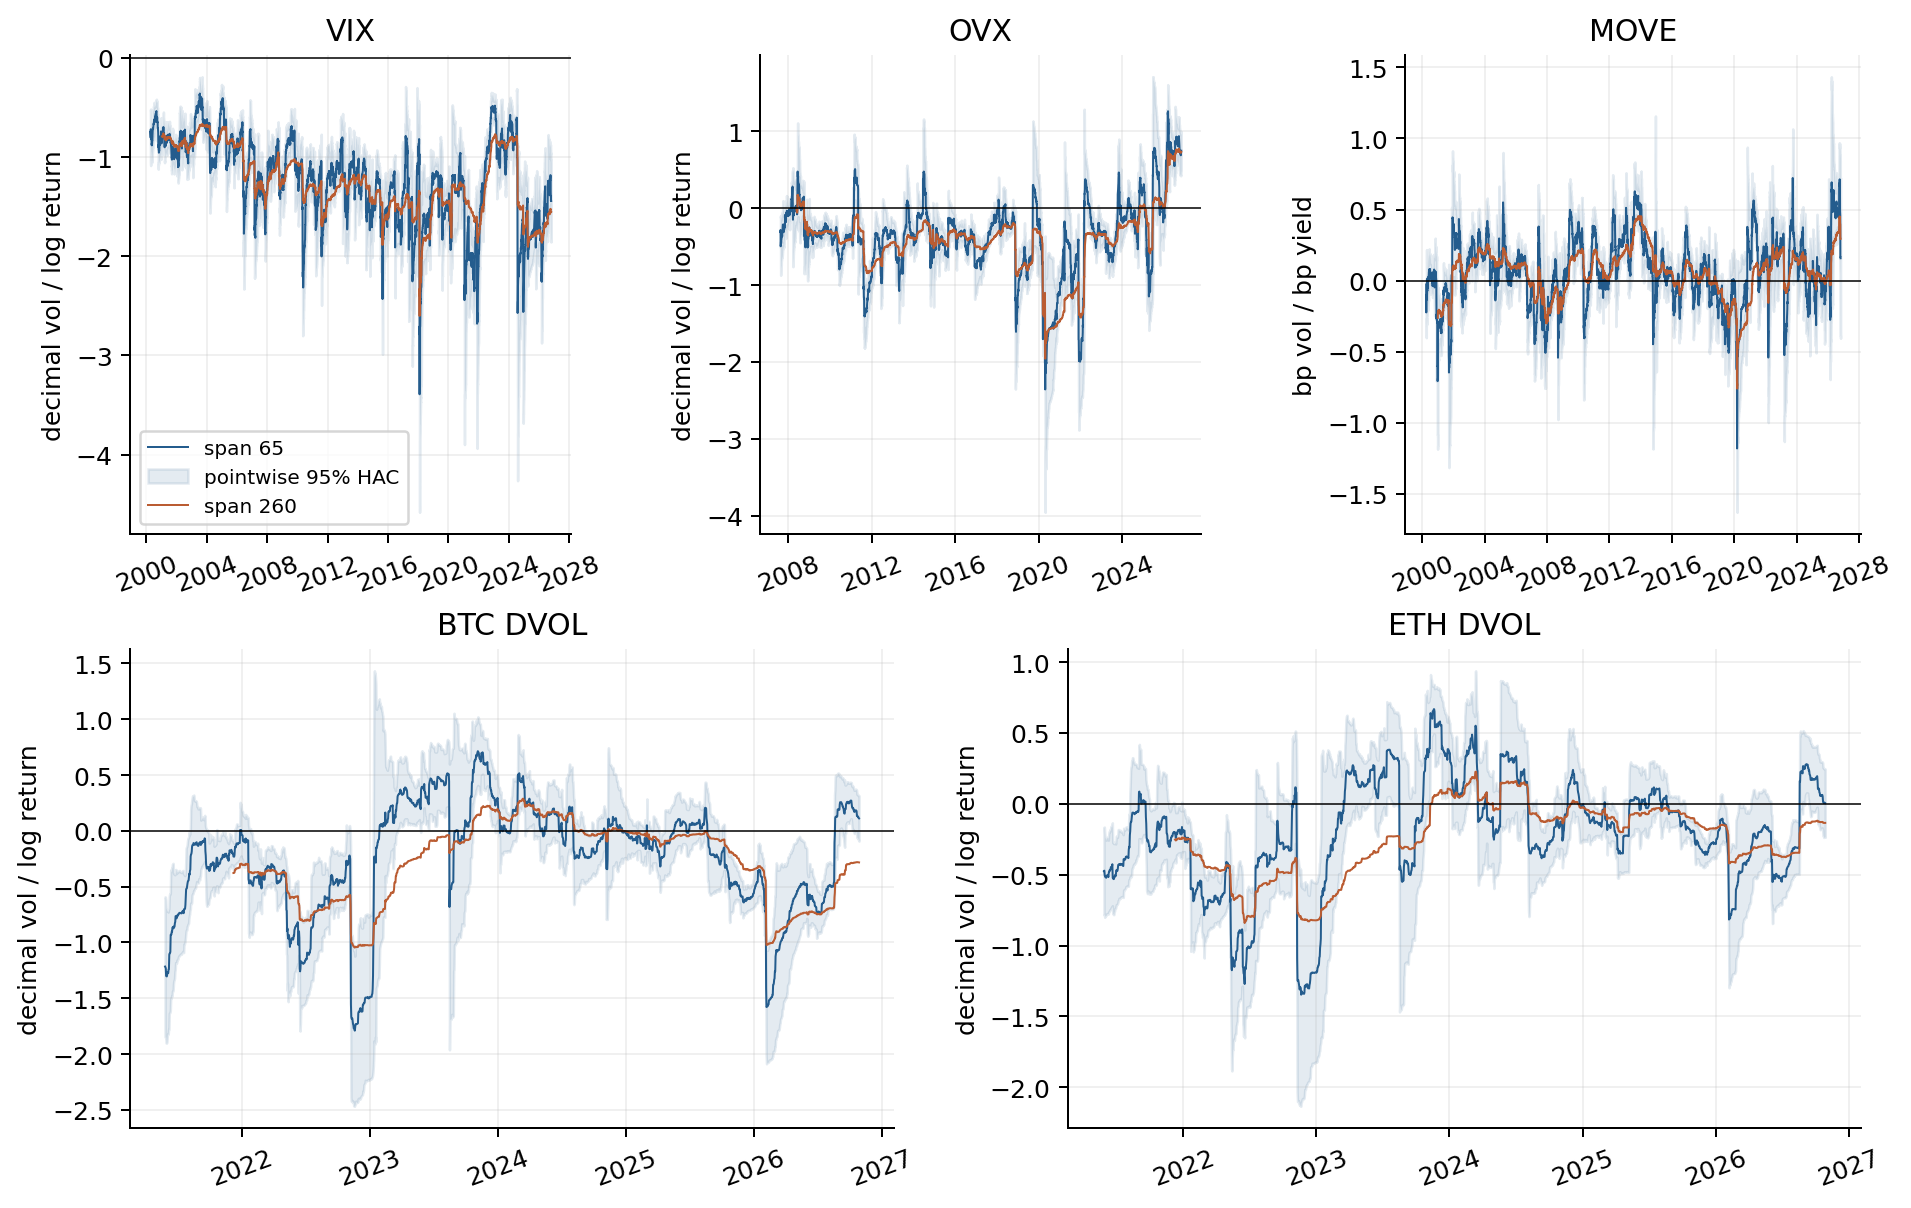
\includegraphics[width=\textwidth,height=.55\textheight,keepaspectratio]{figures/empirical_bloomberg_20261030/beta_five.png}
\caption{Observed level-beta paths for VIX, OVX and MOVE (top) and for BTC and ETH DVOL (bottom). Blue: span 65 with pointwise 95\% Newey--West bands. Orange: span 260. MOVE is bp of yield volatility per bp of yield change, and the other slopes are decimal volatility per log return. Bloomberg spans count retained sessions, DVOL spans count calendar days, and DVOL dates label the candle start. Sources: Bloomberg, 2000--2026, and Deribit, 24 March 2021 to 28 October 2026.}\label{fig:observed-beta}\end{figure}

% [AI-DRAFT BEGIN: Cboe panel paragraph, condensed from the 29 Oct draft.]
Cboe's named volatility indices extend the comparison to fifteen established
price-volatility histories with a common 30-day target, selected from the index
methodology before any outcome was examined.\footnote{Cboe Selected Broad-Based
Index, Equity and ETF Volatility Indices, version 9.0, 30 March 2026:
\url{https://cdn.cboe.com/api/global/us_indices/governance/Volatility_Index_Methodology_Selected_Broad_Based_Index_Equity_and_ETF_Volatility_Indices.pdf}.
Newer and relaunched candidates are inventoried in the replication package and are not pooled.}
Native histories can contain pre-launch calculated values, so Table~\ref{tab:cboe-panel}
also reports the common post-launch sample of 2898 sessions from 2015-04-22 to 2026-10-28.
Single-stock indices add firm-specific variation that a daily panel does not
isolate, and correlated markets share shocks, so the fifteen series are not
fifteen independent replications. The table also carries the held-out GIG-minus-Heston
log scores of Section~\ref{sec:empirical-density} on the native histories. The
common-session scores and the span-260 fractions are in the replication package.
% [AI-DRAFT END]

{\small\setlength{\tabcolsep}{3pt}\begin{longtable}{@{}l P{22mm} l r r r r r l@{}}\caption{Established Cboe volatility-index panel. Positive-beta columns are percentages of days at span 65 on the native history and on the common post-launch sessions. ACF$_{63}$ is the lag-63 level correlation. Score is the held-out GIG minus Heston-marginal mean log score on the native history, with its pointwise 95\% circular-block interval (65 observations), from a chronological 70/30 split per series with the training fit held fixed. The intervals come from a separate resampling run with its own seed, so the VIX and OVX intervals differ by resampling error from those of Table~\ref{tab:empirical-scores}. Source: Bloomberg, with all histories ending on 28 October 2026.}\label{tab:cboe-panel}\\\toprule Index & Reference & First value & $N$ & Native $+$ & Common $+$ & ACF$_{63}$ & Score & 95\% interval\\\midrule\endfirsthead\toprule Index & Reference & First value & $N$ & Native $+$ & Common $+$ & ACF$_{63}$ & Score & 95\% interval\\\midrule\endhead

VIX & SPX & 2000-01-03 & 6779 & 0.0 & 0.0 & 0.521 & 0.163 & [0.053, 0.287] \\

OVX & USO & 2007-05-10 & 4903 & 17.0 & 21.4 & 0.307 & 0.083 & [-0.023, 0.192] \\

RVX & RTY & 2004-01-02 & 5740 & 0.1 & 0.2 & 0.541 & 0.059 & [-0.046, 0.180] \\

VXN & NDX & 2001-02-02 & 6475 & 0.0 & 0.0 & 0.707 & 0.135 & [0.052, 0.218] \\

VXD & INDU & 2000-01-03 & 6750 & 0.7 & 1.8 & 0.527 & 0.169 & [0.062, 0.295] \\

GVZ & GLD & 2008-06-03 & 4634 & 53.4 & 66.4 & 0.600 & 0.136 & [0.047, 0.209] \\

VXEEM & EEM & 2011-03-16 & 3929 & 2.1 & 2.9 & 0.317 & 0.113 & [0.028, 0.184] \\

VXEFA & EFA & 2008-01-02 & 4736 & 0.7 & 0.9 & 0.517 & 0.234 & [0.150, 0.310] \\

VXEWZ & EWZ & 2011-03-16 & 3929 & 2.4 & 0.9 & 0.323 & 0.153 & [0.079, 0.216] \\

VXTLT & TLT & 2004-01-02 & 5733 & 46.3 & 43.1 & 0.578 & 0.043 & [-0.123, 0.352] \\

VXAPL & AAPL & 2011-01-07 & 3975 & 4.3 & 0.8 & 0.361 & 0.072 & [0.012, 0.131] \\

VXAZN & AMZN & 2011-01-07 & 3975 & 12.8 & 7.6 & 0.540 & -0.002 & [-0.020, 0.016] \\

VXGOG & GOOG & 2011-01-07 & 3975 & 7.5 & 8.2 & 0.531 & -0.072 & [-0.126, -0.012] \\

VXGS & GS & 2011-01-07 & 3975 & 0.9 & 1.2 & 0.393 & 0.087 & [0.011, 0.176] \\

VXIBM & IBM & 2011-01-07 & 3975 & 21.5 & 24.5 & 0.570 & 0.080 & [-0.028, 0.233] \\

\bottomrule\end{longtable}}

\subsection{Stationary marginals and chronological transfer}
\label{sec:empirical-density}
% [AI-DRAFT BEGIN: marginal-fit findings with the 3/2 family, 30 Oct 2026. Author pass pending.]
Marginal transfer depends on the asset and the evaluation period. VIX favours the
GIG family over the Heston marginal with an interval above zero, OVX favours it as
a point estimate, MOVE does not, and DVOL separates the two heavy-tailed families.
We fit four stationary
families to the first 70\% of each history by maximum likelihood and evaluate the
mean log score on the last 30\%: the GIG law in volatility, including its exact
Gamma and inverse-Gamma limits, the Heston marginal $2s\,p_V(s^2)$ with $V$ Gamma,
the 3/2 marginal $2s\,p_V(s^2)$ with $V$ inverse-Gamma, and the lognormal law.
Table~\ref{tab:empirical-scores} reports the held-out differences in favour of the
GIG candidate. Against the Heston marginal the VIX difference is 0.163 with
a block interval above zero, and the score column of Table~\ref{tab:cboe-panel}
is positive for 13 of 15 indices, with 9 intervals above zero and 1 below. Against the 3/2 marginal the VIX difference is -0.009, with an
interval that contains zero, so the two power-tailed laws are indistinguishable on
this criterion. Figure~\ref{fig:observed-density} shows the fitted survival
functions against the held-out Bloomberg tails.

The two DVOL training fits select interior GIG laws. On BTC DVOL, GIG-minus-Heston
and GIG-minus-3/2 scores are \scoreBTCDVOLHeston\ and \scoreBTCDVOLThreeHalf,
with both intervals including zero. On ETH DVOL, the corresponding differences are
\scoreETHDVOLHeston\ and \scoreETHDVOLThreeHalf, and both intervals exclude zero, so
ETH DVOL favours GIG against Heston and the 3/2 marginal against GIG. ETH also favours the
lognormal law over GIG. Thus there is no common winning marginal family across
the five indices. Both crypto evaluation samples have no observation above their
own training 95th percentile, so this is transfer to a lower-volatility period
and not a stress-tail validation. DVOL survival plots and persistence diagnostics are
in the replication package.

The fitted GIG law selects its inverse-Gamma limit, the boundary $C=0$ of
Proposition~\ref{prop:stationary}, for VIX and OVX, and an
interior law for MOVE, BTC DVOL, ETH DVOL. An index marginal is the law of
$F(\sigma)$ rather than of $\sigma$, so the VIX and OVX fits do not estimate the latent
physical drift. The index fits motivate examining the inverse-Gamma boundary,
without identifying $C_P=0$ for latent volatility. If a separately estimated latent
physical model has $C_P=0$, then~\eqref{eq:pq-map} gives
$C_Q=\beta\ell_0+\varepsilon\ell_1$. A valid pricing density and stock martingality
jointly require the projected risk price to satisfy
$\beta\ell_0+\varepsilon\ell_1\geq\max(\beta,0)$.
For $\beta>0$, this requires a positive quadratic coefficient under the pricing
measure, although $C_Q\geq\beta$ need not hold with equality. This conditional
model construction is distinct from an inference about latent dynamics from
the index marginals.

For a fitted inverse-Gamma index law with shape $\alpha>0$, positive moments of
order $r$ are finite if and only if $r<\alpha$, and diverge for $r\geq\alpha$.
The fitted shapes are about 8 for both series, so the fitted index laws have finite
moments up to order seven and divergent moments above order eight.

These are comparisons of marginal families on an observed index, not of calibrated
dynamic models. Normalisation uses the training median only, score intervals hold
the training fit fixed, and the single chronological split is descriptive.
% [AI-DRAFT END]

\begin{table}[htbp]\centering\small\setlength{\tabcolsep}{3pt}\begin{tabular}{@{}l P{24mm} P{36mm} P{36mm} P{36mm}@{}}\toprule Series & GIG law & GIG minus Heston & GIG minus 3/2 & GIG minus lognormal\\\midrule

VIX & Inverse-Gamma & 0.163 [0.049, 0.269] & -0.009 [-0.036, 0.013] & 0.028 [-0.001, 0.059] \\

OVX & Inverse-Gamma & 0.083 [-0.022, 0.183] & 0.027 [0.006, 0.051] & -0.005 [-0.034, 0.023] \\

MOVE & Interior GIG & -0.035 [-0.115, 0.045] & 0.043 [0.010, 0.077] & -0.026 [-0.054, -0.000] \\

BTC DVOL & Interior GIG & 0.028 [-0.044, 0.097] & 0.036 [-0.048, 0.128] & 0.007 [0.002, 0.012] \\

ETH DVOL & Interior GIG & 0.081 [0.059, 0.105] & -0.093 [-0.167, -0.021] & -0.036 [-0.050, -0.024] \\

\bottomrule\end{tabular}\caption{Held-out mean log-score differences in favour of the selected GIG candidate, with pointwise 95\% circular-block intervals (65 observations, 400 resamples). Heston denotes the square-root-Gamma marginal and 3/2 the square-root-inverse-Gamma marginal. Training on the first 70\% of each history, evaluation on the last 30\%. Sources: Bloomberg and Deribit, with coverage in Table~\ref{tab:empirical-data}.}\label{tab:empirical-scores}\end{table}

\begin{figure}[tbp]\centering
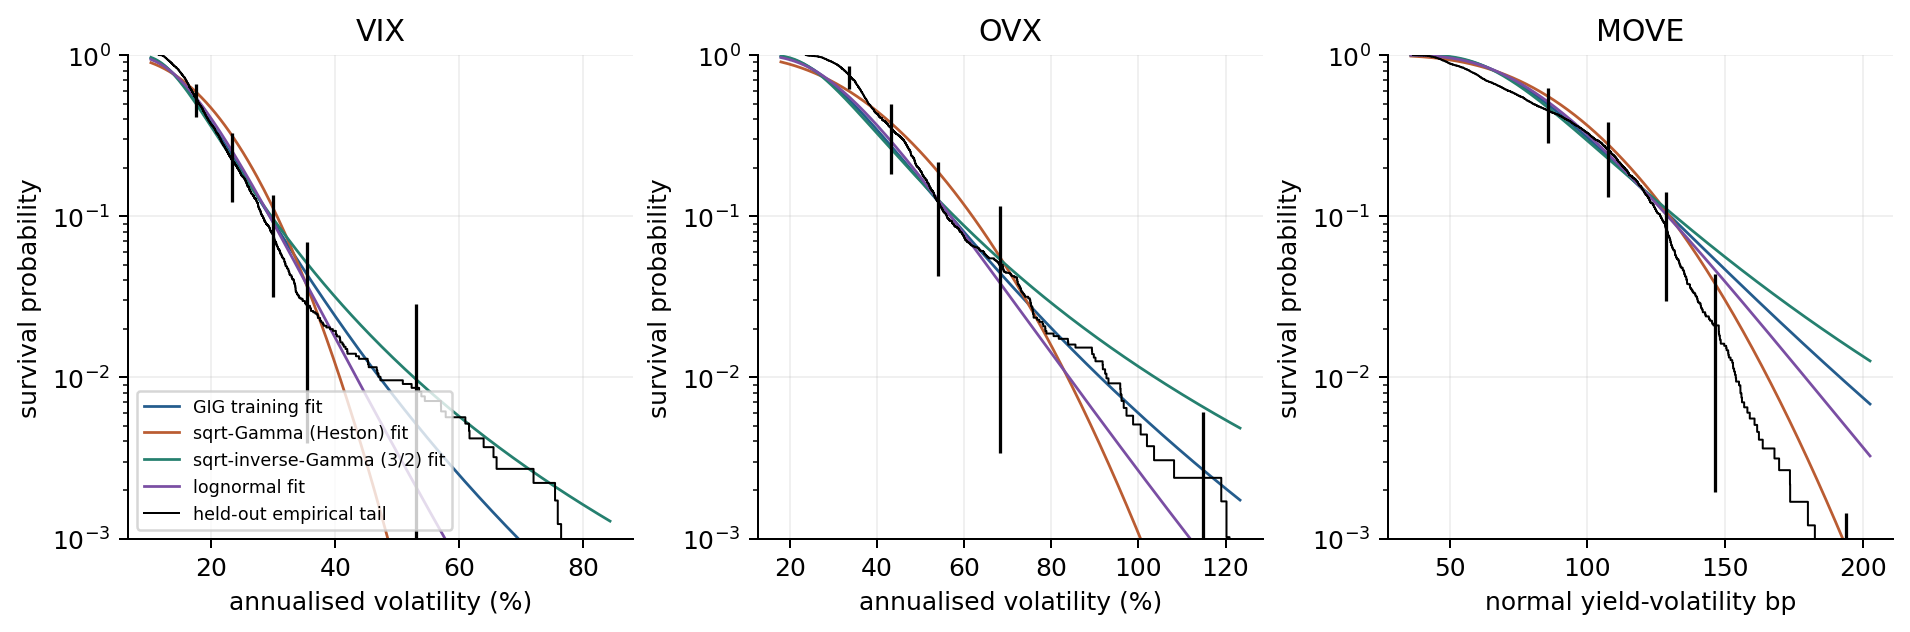
\includegraphics[width=\textwidth,height=.4\textheight,keepaspectratio]{figures/empirical_bloomberg_20261030/density_main.png}
\caption{Training-fitted survival functions and held-out empirical tails for VIX, OVX and MOVE. Bars are pointwise block intervals at training quantiles, and the logarithmic axis is truncated below 0.001. Source: Bloomberg, 2000--2026.}\label{fig:observed-density}\end{figure}

\subsection{Observed persistence}
\label{sec:empirical-acf}
% [AI-DRAFT BEGIN: persistence paragraph, condensed. Author pass pending.]
Lag correlations of the index levels decay slowly and unevenly across assets.
At lag 120 the correlations are VIX: 0.363, OVX: 0.196, MOVE: 0.649, BTC DVOL: 0.703, ETH DVOL: 0.600, and the lag-63 values of the Cboe panel in
Table~\ref{tab:cboe-panel} range from 0.31 (OVX) to 0.71 (VXN). We compute Pearson correlations of lagged level pairs at lags 1 to 120
observations, with circular blocks of 250 observations resampling the lag-pair
vectors. The correlation paths and their pointwise block intervals are in the
replication package. These diagnostics assume a stationary approximation despite visible regime
changes. They do not identify roughness or the latent mean-reversion clock, for the
two reasons developed in Section~\ref{sec:observations}: the observable is a map of
the state, and finite samples can bias an ACF estimator. The synthetic study below
illustrates this bias using a full-sample-centred estimator. Its centring and
variance normalisation differ from the lag-pair Pearson estimator used here,
so its bias values do not quantify the bias of these empirical estimates.
% [AI-DRAFT END]

\subsection{Synthetic observation maps and finite-sample persistence}
\label{sec:synthetic-observation-acf}
% [AI-DRAFT BEGIN: updated VIX calibration and synthetic results. Author pass pending.]
We fit the quadratic-drift model to 6,779 daily Bloomberg VIX closes
from January 2000 through October 2026 (Table~\ref{tab:empirical-data}).
For each pair $(\kappa_1,\kappa_2)$, we choose $\theta$ and total volatility of volatility $v$
by matching the stationary log-volatility density to a 50-bin histogram of $\log(\mathrm{VIX}/100)$.
We then choose $(\kappa_1,\kappa_2)$ by matching daily VIX level
autocorrelations at lags 1 to 119. Both steps minimise sums of squared errors.
For each pair we average the model autocorrelations over 10,000 ten-year paths with common random shocks.
The fitted index coefficients are $(\theta,\kappa_1,\kappa_2,v)=(0.1995,0.2000,9.1829,0.6851)$.
The estimate of $\kappa_1$ reaches its lower search bound of $0.2$.

We use these coefficients for the latent state in a synthetic observation experiment.
The two Brownian loadings enter the index dynamics only through $v^2=\beta^2+\varepsilon^2$. We choose $\beta=0.35$
for illustration and set the residual loading to $\sqrt{v^2-\beta^2}$.
We set $Q=P$ to isolate the observation map $F_\tau(\sigma)$, the ideal
variance-swap volatility at $\tau=30/365$ years.

The stationary mean and standard deviation are 0.17967
and 0.06326 for latent volatility and 0.18125 and
0.05856 for the mapped index. At the stationary median
$\sigma=0.17142$, the map gives $F_\tau(\sigma)=0.17479$.
The instantaneous index-level beta is $\beta F_\tau'(\sigma)=0.33076$.
The 30-day observation horizon thus changes both the stationary distribution
and the return sensitivity even when $Q=P$.
% [AI-DRAFT END]

We multiply $(\kappa_1,\kappa_2,v^2)$ by clocks $c=1$ and $c=0.25$,
holding $\theta$ fixed and multiplying $\beta$ by $\sqrt{c}$.
This preserves the latent invariant distribution while replacing its
population autocorrelation $\rho(h)$ by $\rho(ch)$.
We recompute the fixed-maturity observation map for each clock.
For each regime, 400 independent paths start from the invariant GIG distribution.
We record 252 observations per model year with four positive splitting steps per observation.
The sample ACF uses the full-sample mean. At lag $h$ we divide the cross-product
sum by $N-h$ and the sum of squared deviations by $N$.
Table~\ref{tab:synthetic-acf-bias} reports the bias at lag 63.
Figure~\ref{fig:synthetic-acf-bias} shows its lag profile.

\begin{table}[htbp]\centering\small
\begin{tabular}{rrrrrr}\toprule
Clock & Years & Population ACF & Mean sample ACF & Bias & MC s.e.\\
\midrule

1.00 & 5 & 0.5991 & 0.4481 & -0.1509 & 0.0080 \\

1.00 & 10 & 0.5991 & 0.5260 & -0.0731 & 0.0061 \\

1.00 & 20 & 0.5991 & 0.5698 & -0.0293 & 0.0041 \\

0.25 & 5 & 0.8767 & 0.6366 & -0.2402 & 0.0088 \\

0.25 & 10 & 0.8767 & 0.7560 & -0.1207 & 0.0057 \\

0.25 & 20 & 0.8767 & 0.8224 & -0.0543 & 0.0034 \\

\bottomrule\end{tabular}
\caption{Synthetic sample-ACF bias at lag 63. Monte Carlo standard errors describe
the estimated mean across independent paths. The three horizons use nested prefixes of each path.}
\label{tab:synthetic-acf-bias}\end{table}

\begin{figure}[htbp]\centering
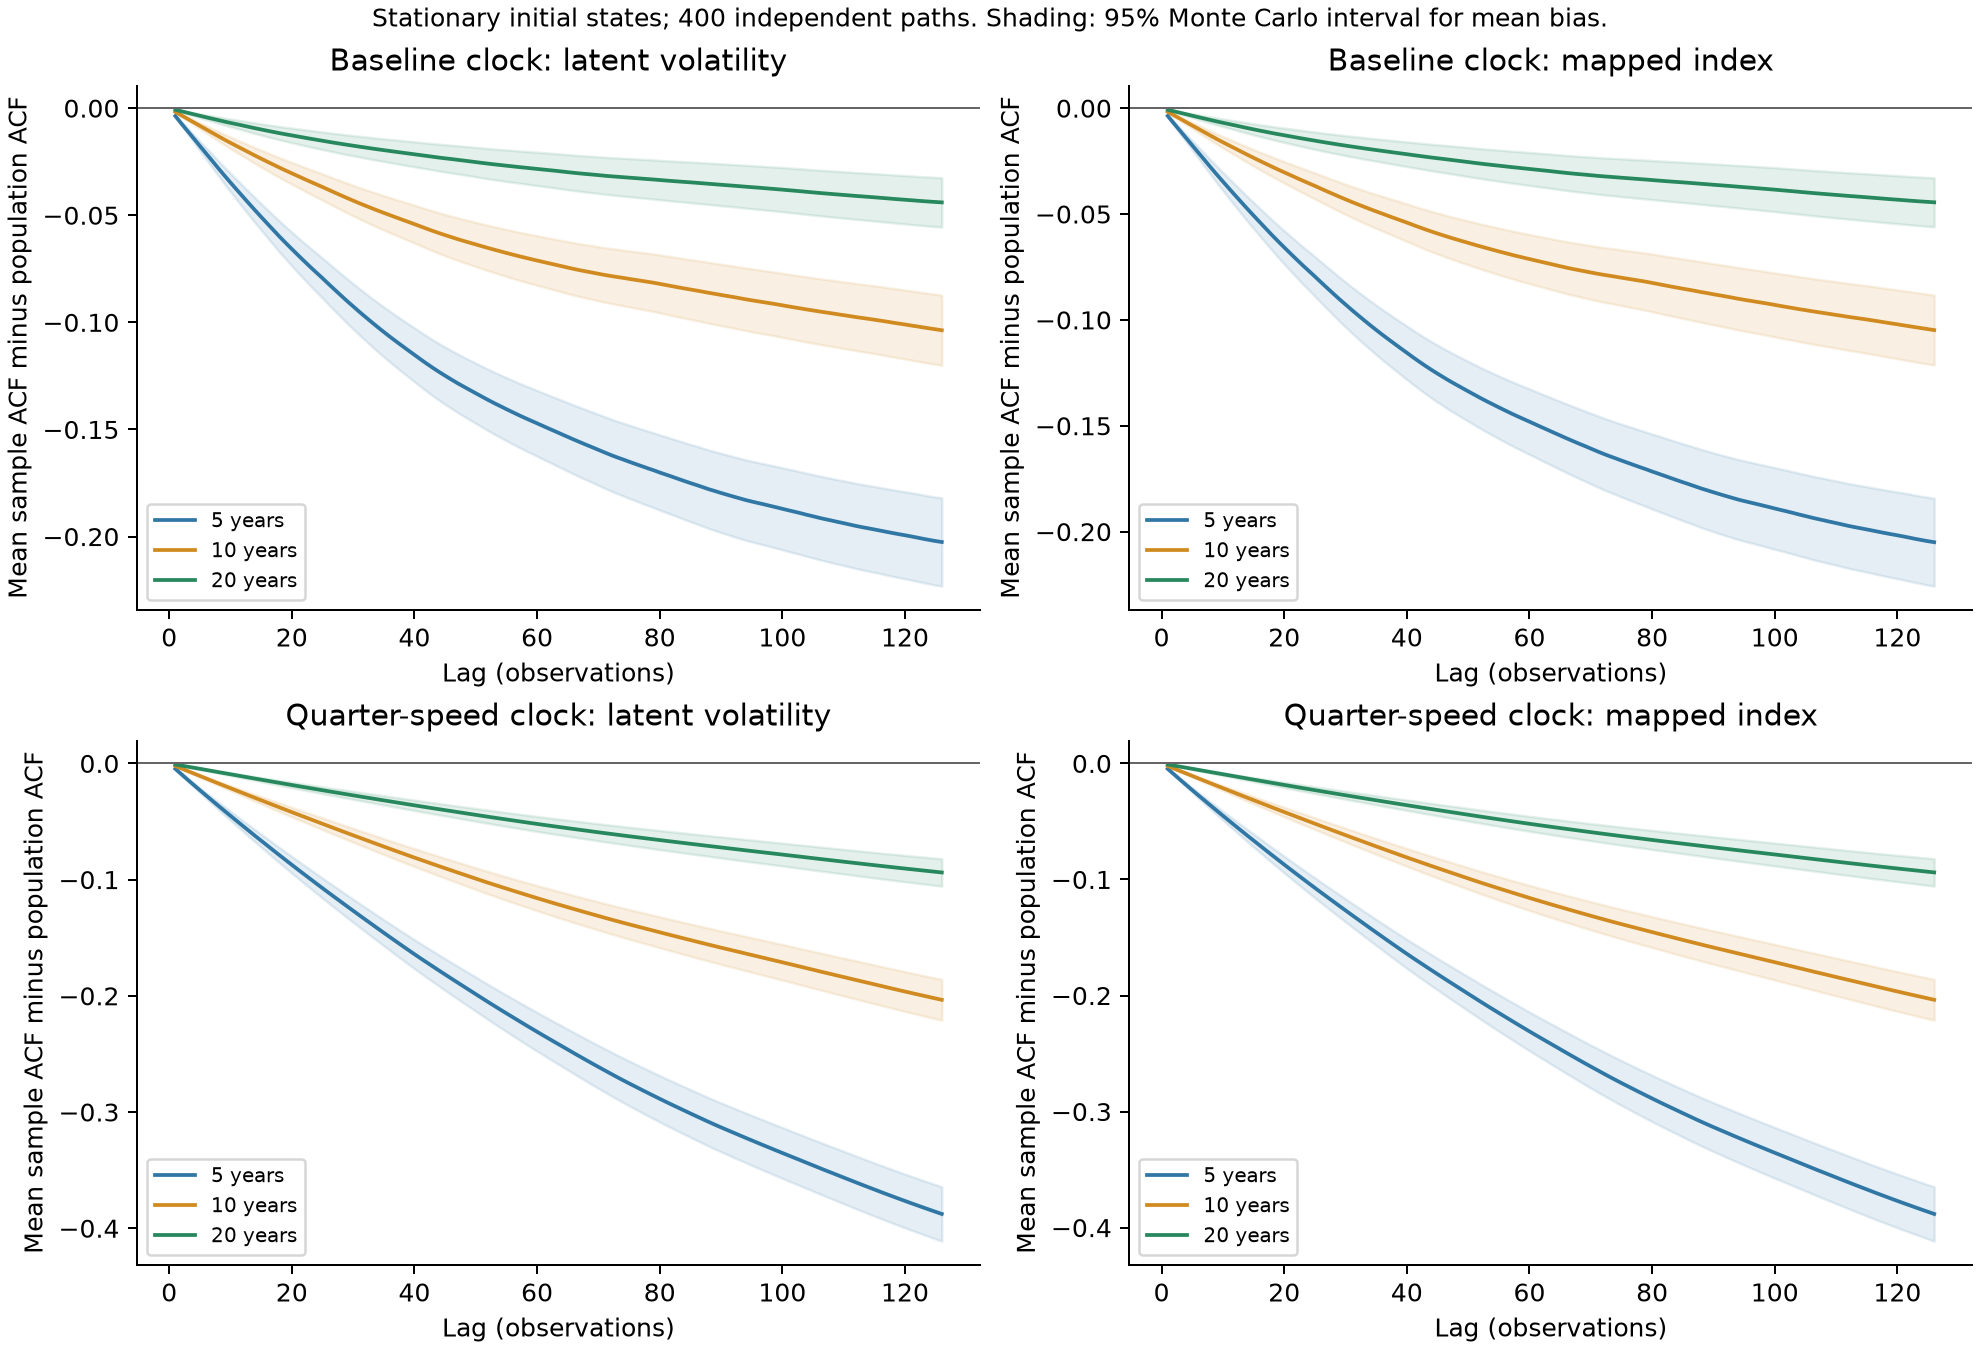
\includegraphics[width=\textwidth,height=.76\textheight,keepaspectratio]{figures/vix_fit_20261123/synthetic_sample_acf_bias.png}
\caption{Average sample-ACF bias for latent and mapped volatility under the two clocks. Shading gives 95\% Monte Carlo intervals for the mean bias.}\label{fig:synthetic-acf-bias}\end{figure}

We compute the observation map and population ACF with a reversible
finite-volume generator on a log-volatility grid. When we double the daily splitting steps
from four to eight, the largest absolute change in the mean latent sample ACF is approximately
$7.5\times 10^{-6}$ across lags 0 to 126.
The replication package also reports grid refinement and independent Monte Carlo checks.

\subsection{Reproducibility and scope}
% [AI-DRAFT BEGIN: scope paragraph, condensed. Author pass pending.]
The replication package\footnote{\url{https://github.com/ArturSepp/StochVolModels},
directory \path{papers/robust_volatility_models_2026/replication}. Code, the Cboe-index pipeline,
quote hashes and every fitted parameter are included. Bloomberg and ThetaData
inputs are licensed and are not included.} stores the inputs, seeds,
results and figures of this section, the synthetic study, and the option-surface
calibrations of Section~\ref{sec:oca-calibration}. The single chronological split
is descriptive, and the block intervals describe sampling error under a stationary
approximation. Joint estimation of latent dynamics from realised and implied
volatility is a separate project.
% [AI-DRAFT END]


% Generated by calibration_section_20261030/make_calibration_section.py from the frozen
% calibration_pde_20261029 and calibration_positive_skew_20261031 outputs. No recalibration.
% AI-DRAFT blocks await the author's pass.
\subsection{Four-maturity calibrations on four option snapshots}
\label{sec:oca-calibration}
% [AI-DRAFT BEGIN: calibration data and conventions, rewritten point-first, 30 Oct 2026.]
We calibrate Heston and quadratic-drift LogSV jointly to four maturities of three
option surfaces observed on 15 July 2026: SPXW (weekly S\&P~500 index options), GLD
(options on the SPDR gold ETF) and TLT (options on the iShares 20+ year Treasury
bond ETF). The quotes are
ThetaData end-of-day option chains processed with the \texttt{option-chain-analytics}
package (OCA),\footnote{\url{https://github.com/ArturSepp/OptionChainAnalytics}. OCA
supplies the cached parity-implied forwards and discounts, the bid and ask implied
volatilities and the exact maturities used here. The report timestamps are
retained and are not synchronous closing executions.} which also supplies the
forward, discount and implied-volatility conventions. SPXW is the European
benchmark. GLD and TLT options are American, and for them OCA reports
European-equivalent Black implied volatilities, so the ETF examples compare smiles
under that convention and are not exact American-option prices. For each slice OCA
fits the European parity line $C-P=D(F-K)$ across strikes for the forward $F$ and
the discount $D$ and inverts the Black formula at these values, with no adjustment
for early exercise.
% [AUTHOR: the sentence above describes option-chain-analytics 6.0.2 (data/thetadata.py and
%  utils/forward_discount.py). Confirm that the cached surfaces were built with this routine.]
The ETF parity-implied
discounts exceed one in these slices and are normalisation inputs, not risk-free
curve estimates. Each surface uses the 27 July 2026 expiry (about 12 days) and
three further expiries: 14 August, 18 September and 16 October for SPXW and GLD
(about 30, 65 and 93 days), and 14, 21 and 28 August for TLT (about 30, 37 and 44
days). After the filters (positive ordered premiums, $|\log(K/F)|\leq0.15$, bid--ask
IV spread at most three volatility percentage points, at most 25 evenly spaced
strikes per slice plus the nearest ATM strike) the samples contain 103, 102 and 89
out-of-the-money quotes. All twelve slices have negative 25-delta smile skew, an
observable that is distinct from a fitted latent $\beta$.

A fourth snapshot, TLT on 2 August 2024 (denoted TLT+), exercises positive smile
skew with the same filters, objective, bounds and numerical checks. Its 99 quotes
span expiries 14 August, 30 August, 20 September and 30 September 2024 (about
12, 28, 49 and 59 days), and all four slices have positive 25-delta smile skew.
The candidate search tried GLD first, then TLT, requiring four usable maturities
and a positive 30-day skew, and the strict all-four-positive rule was not relaxed.
The selected snapshot maximises the 30-day skew among eligible TLT candidates.
The GLD archive holds 22 dates, all in July 2026, and no qualifying positive
30-day skew, whereas the TLT archive has 805 dates from June 2023 to August 2026, of which
196 have positive 30-day skew. This unequal coverage and the deliberate extreme
selection make TLT+ a methodological illustration, not an estimate of positive-skew
frequency across markets. The shorter expiry is retained in both models' joint fits.
% [AI-DRAFT END]

\paragraph{Objective and numerical implementation.}
The objective gives equal weight to each maturity and equal weight to retained
strikes within each maturity, and it targets the midpoint of bid and ask IVs.
For a parameter vector $\Theta$, $M=4$ maturities and $n_i$ retained strikes at maturity
$i$, define the decimal-IV residual
$e_{ij}(\Theta)=\sigma^{\mathrm{model}}_{ij}(\Theta)
-(\sigma^{\mathrm{bid}}_{ij}+\sigma^{\mathrm{ask}}_{ij})/2$. We minimise
\begin{equation}
 J(\Theta)=\frac{1}{M}\sum_{i=1}^{M}\frac{1}{n_i}\sum_{j=1}^{n_i}e_{ij}(\Theta)^2,
 \qquad \mathrm{RMSE}_{\mathrm{pp}}=100\sqrt{J(\Theta)}.
 \label{eq:oca-calibration-objective}
\end{equation}
Here $\mathrm{RMSE}_{\mathrm{pp}}$ is the root-mean-square error (RMSE) in volatility
percentage points (pp). Heston has five fitted parameters and LogSV six, and one
parameter vector fits all four maturities. We impose positive levels and drift
speeds and Heston $|\rho|<1$. For LogSV we fit the margin
$m=\kappa_2-\max(\beta,0)$ with $m\geq0.05$, which keeps $\kappa_2\geq0$ and
$\kappa_2\geq\beta$, the domain of Proposition~\ref{prop:martingale}, with a
numerical buffer. Heston's Feller condition is not imposed.

Heston uses its transform kernel, and every price is rechecked against a separately
coded characteristic function with adaptive quadrature. LogSV is calibrated with
the full-state backward transform PDE in log volatility, followed by Fourier
inversion, which retains the volatility-state dependence without truncating the
log transform to a finite polynomial.
Under the money-market measure, we use the
zero-carry normalisation $X_t=\log(S_t/S_0)$, so $X_0=0$.
For $y=\log\sigma$, $v^2=\beta^2+\varepsilon^2$ and
$U(t,y;\phi)=\E[\exp(-\phi X_t)\mid\sigma_0=e^y]$, the equation is
\begin{align}
 \partial_t U &= \tfrac12v^2\partial_{yy}U
   +\bigl[a(y)-\phi\beta e^y\bigr]\partial_yU
   +\tfrac12\phi(\phi+1)e^{2y}U, \qquad U(0,y;\phi)=1,
   \label{eq:oca-transform-pde}\\
 a(y)&=\kappa_1\theta e^{-y}+\kappa_2\theta-\kappa_1
       -\kappa_2e^y-\tfrac12v^2.\nonumber
\end{align}
Here $\Re\phi=-1/2$ is the valuation contour. The model is the Markovian specification
with a flat volatility backbone.
% [AI-DRAFT BEGIN: discretisation of the transform PDE, 17 Nov 2026, second pass. Taken from logvol_pde.py.]
The solver discretises $y$ on a uniform grid with spacing $\Delta y$, centred at
$\log\sigma_0$. It uses central differences, with the diffusion coefficient raised to
$\Delta y\,|a(y)|/2$ at nodes where that value exceeds $v^2/2$. The remote values are one at low volatility and zero at high
volatility. Two implicit Euler half steps precede the Crank--Nicolson steps and damp the
mismatch between the initial condition and the upper remote value.
% [AI-DRAFT END]

Two bounded coarse-grid optimisations use 401 state nodes and 256 time steps, one
started from a simulation-based fit and one from an independent starting
vector. The better solution is refined with 801 nodes and 512 steps. All optimiser
stages terminate successfully, which does not establish a global optimum. Reported
curves and scores use 1601 nodes and 1024 steps, with 64-point Gauss--Legendre
integration in each of six Fourier subintervals up to frequency 1600, on a
log-volatility domain of six units on either side of $\log\sigma_0$.

\begin{table}[htbp]\centering\small
\begin{tabular}{@{}l l r r r r@{}}\toprule
Market & Model & IV RMSE & 12-day RMSE & Inside spread & Fit time\\
 & & (pp) & (pp) & (\%) & (seconds)\\\midrule

SPXW & Heston & 0.698 & 1.127 & 8.7 & 0.16 \\

SPXW & LogSV (PDE) & 0.447 & 0.662 & 20.4 & 268.81 \\

GLD & Heston & 0.477 & 0.446 & 55.9 & 0.23 \\

GLD & LogSV (PDE) & 0.337 & 0.419 & 73.5 & 189.26 \\

TLT & Heston & 0.458 & 0.352 & 37.1 & 0.15 \\

TLT & LogSV (PDE) & 0.295 & 0.274 & 58.4 & 229.15 \\

TLT+ & Heston & 0.796 & 1.223 & 24.2 & 0.13 \\

TLT+ & LogSV (PDE) & 0.585 & 0.837 & 32.3 & 304.14 \\

\bottomrule\end{tabular}
\caption{LogSV lowers the in-sample IV RMSE on all four snapshots at one extra
parameter. Bounded fits to 103 SPXW, 102 GLD and 89 TLT quotes on 15 July 2026.
TLT+ denotes 99 quotes on 2 August 2024, not a second fit to the July TLT snapshot.
The total IV RMSE weights maturities equally, and the 12-day column reports the
shortest slice. Inside-spread percentages count quotes without weights. Heston
times are two-start transform calibrations run separately, and PDE times sum the two coarse
starts and the refinement, excluding simulation-based starting fits, just-in-time compilation warm-up
and validation. Source: ThetaData
via OCA.}
\label{tab:oca-fits}\end{table}

\begin{table}[htbp]\centering\small
\begin{tabular}{@{}l l r r r r r r r r@{}}\toprule
Market & Model & \multicolumn{4}{c}{IV RMSE (pp)} & \multicolumn{4}{c}{Inside spread (\%)}\\
\cmidrule(lr){3-6}\cmidrule(lr){7-10}
 & & 1 & 2 & 3 & 4 & 1 & 2 & 3 & 4\\\midrule

SPXW & Heston & 1.127 & 0.618 & 0.242 & 0.491 & 15 & 4 & 12 & 4 \\

SPXW & LogSV & 0.662 & 0.463 & 0.137 & 0.357 & 15 & 16 & 42 & 8 \\

GLD & Heston & 0.446 & 0.646 & 0.263 & 0.473 & 84 & 27 & 88 & 24 \\

GLD & LogSV & 0.419 & 0.359 & 0.266 & 0.278 & 88 & 69 & 77 & 60 \\

TLT & Heston & 0.352 & 0.515 & 0.445 & 0.503 & 65 & 38 & 33 & 20 \\

TLT & LogSV & 0.274 & 0.334 & 0.272 & 0.295 & 82 & 54 & 57 & 48 \\

TLT+ & Heston & 1.223 & 0.855 & 0.432 & 0.346 & 21 & 16 & 32 & 28 \\

TLT+ & LogSV & 0.837 & 0.682 & 0.355 & 0.277 & 25 & 16 & 48 & 40 \\

\bottomrule\end{tabular}
\caption{LogSV improves 15 of the 16 maturity slices, with the
largest gain at the 12-day SPXW slice. Maturities are numbered from the shortest:
about 12, 30, 65 and 93 days for SPXW and GLD and about 12, 30, 37 and 44 days for
TLT, and about 12, 28, 49 and 59 days for TLT+. Quote counts per slice are 17 to 26.
Source: ThetaData via OCA, with dates as in Table~\ref{tab:oca-fits}.}
\label{tab:oca-maturity}\end{table}

\begin{figure}[tbp]\centering
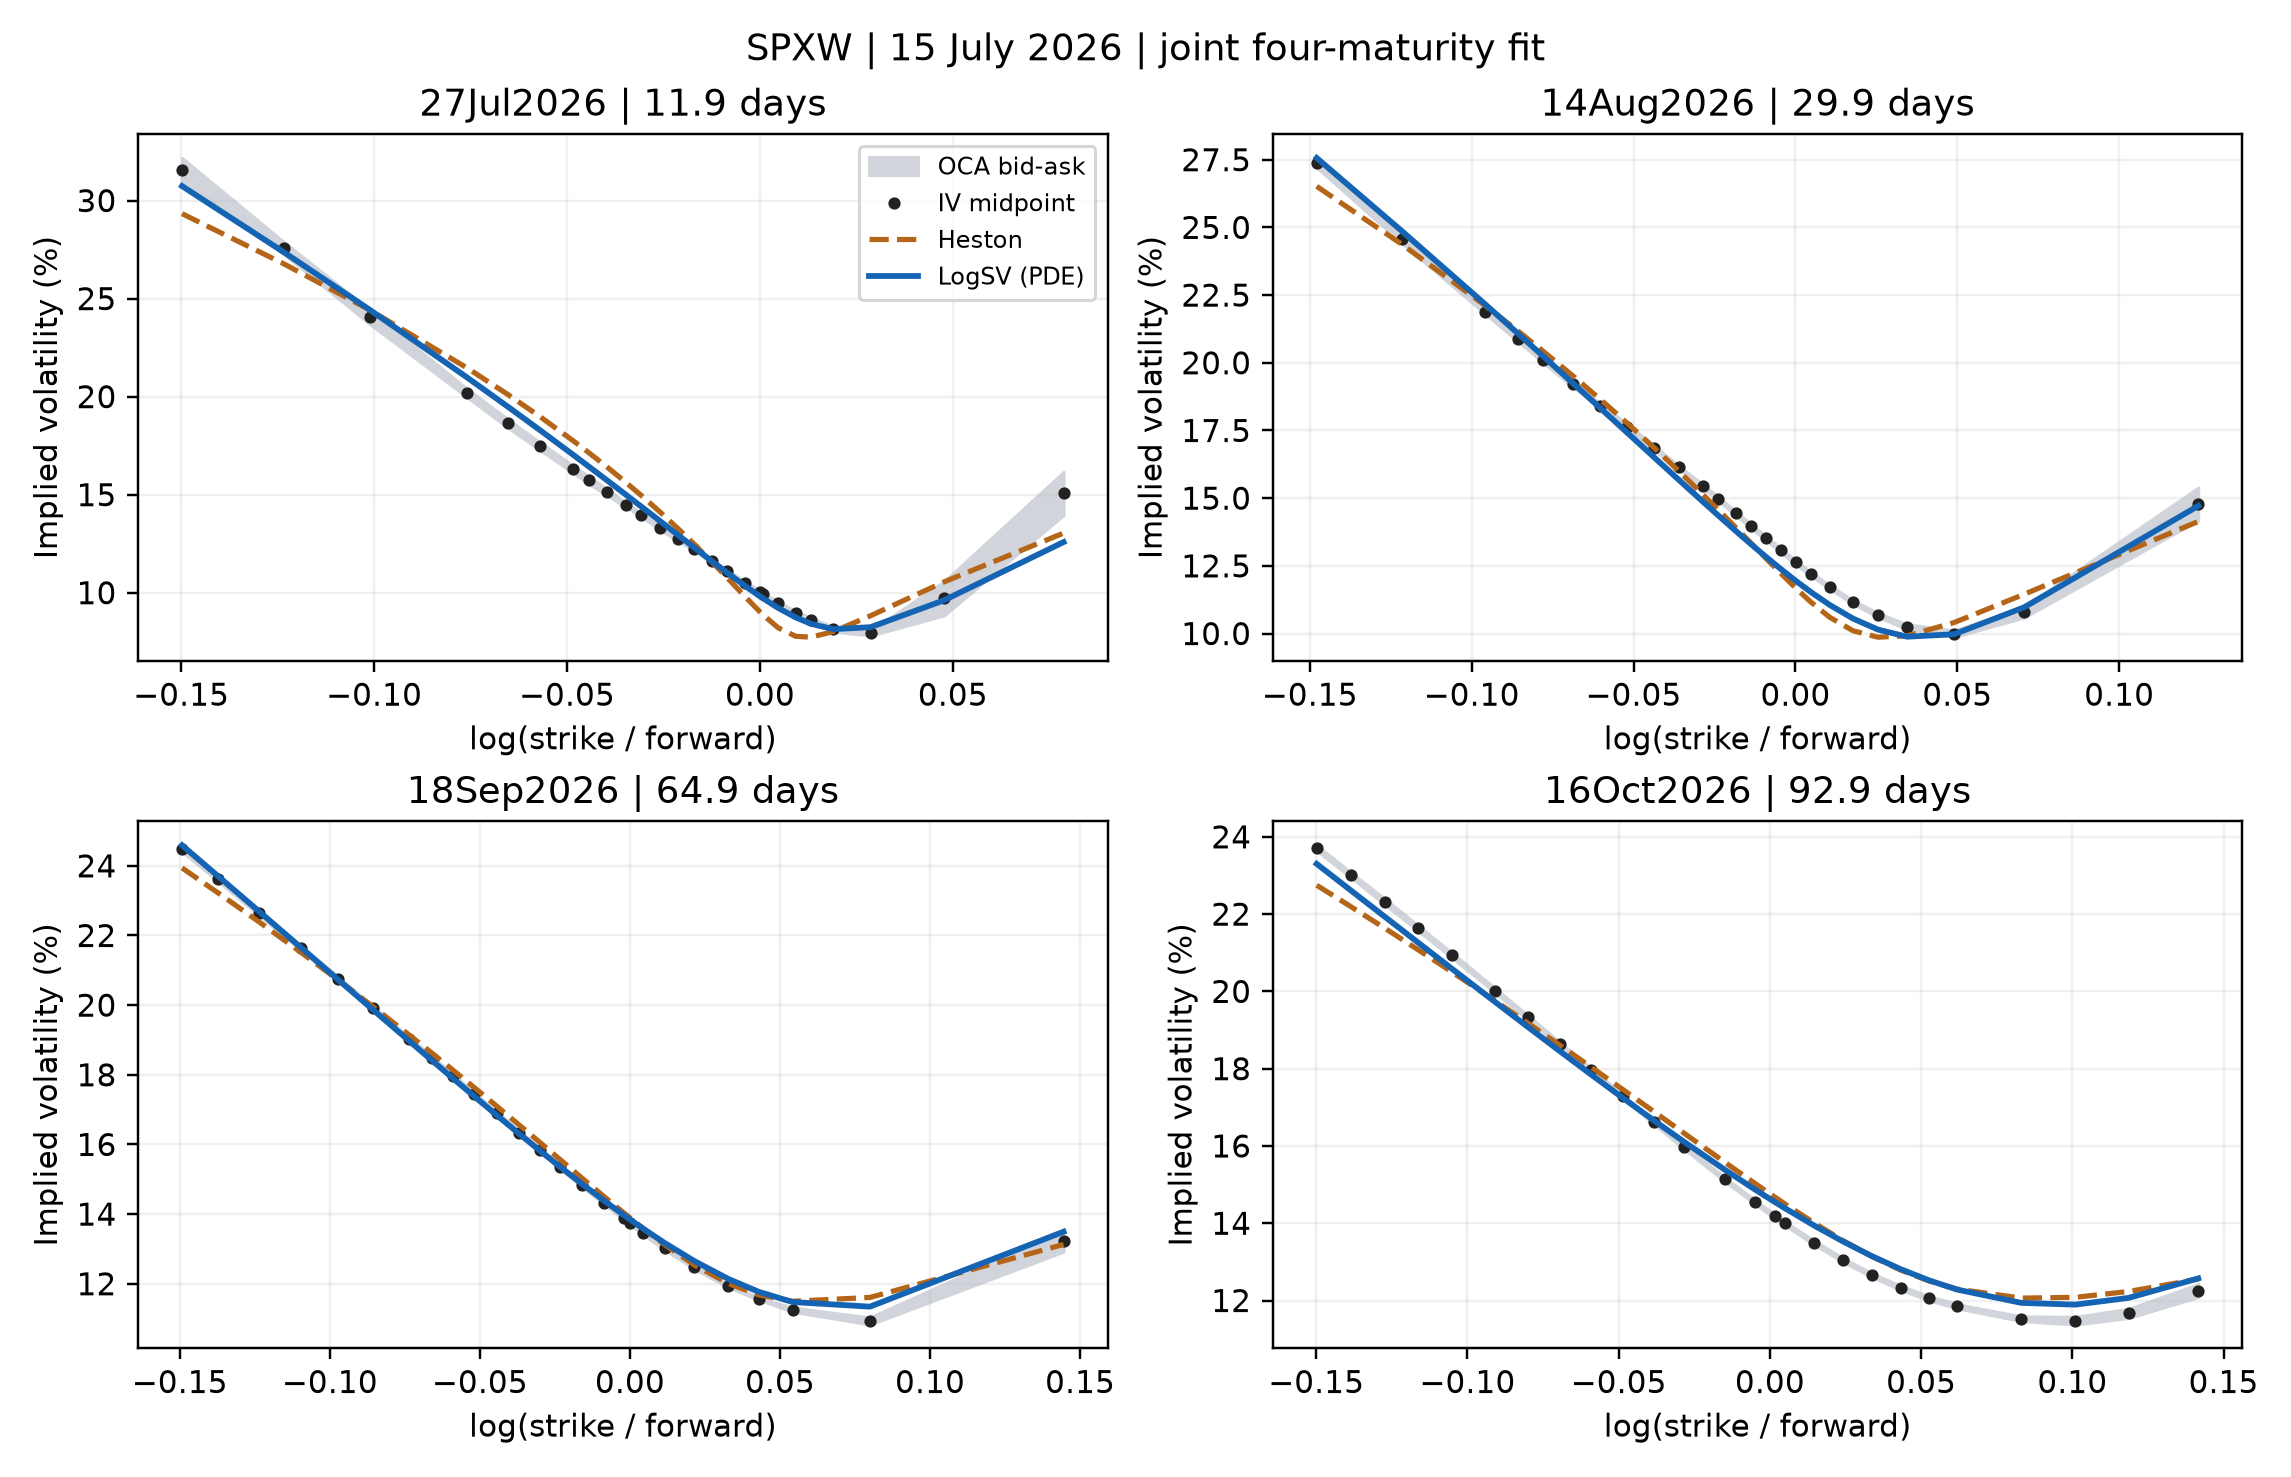
\includegraphics[width=\textwidth]{figures/calibration_pde_20261029/spxw_fits.png}
\caption{SPXW on 15 July 2026, including the approximately 12-day expiry. Points and grey bands show OCA midpoint and bid--ask IVs. The dashed curve is Heston and the solid curve the LogSV fit priced on the fine PDE grid. All four maturities share one parameter vector per model. Source: ThetaData via OCA.}\label{fig:oca-spxw}\end{figure}

\begin{figure}[tbp]\centering
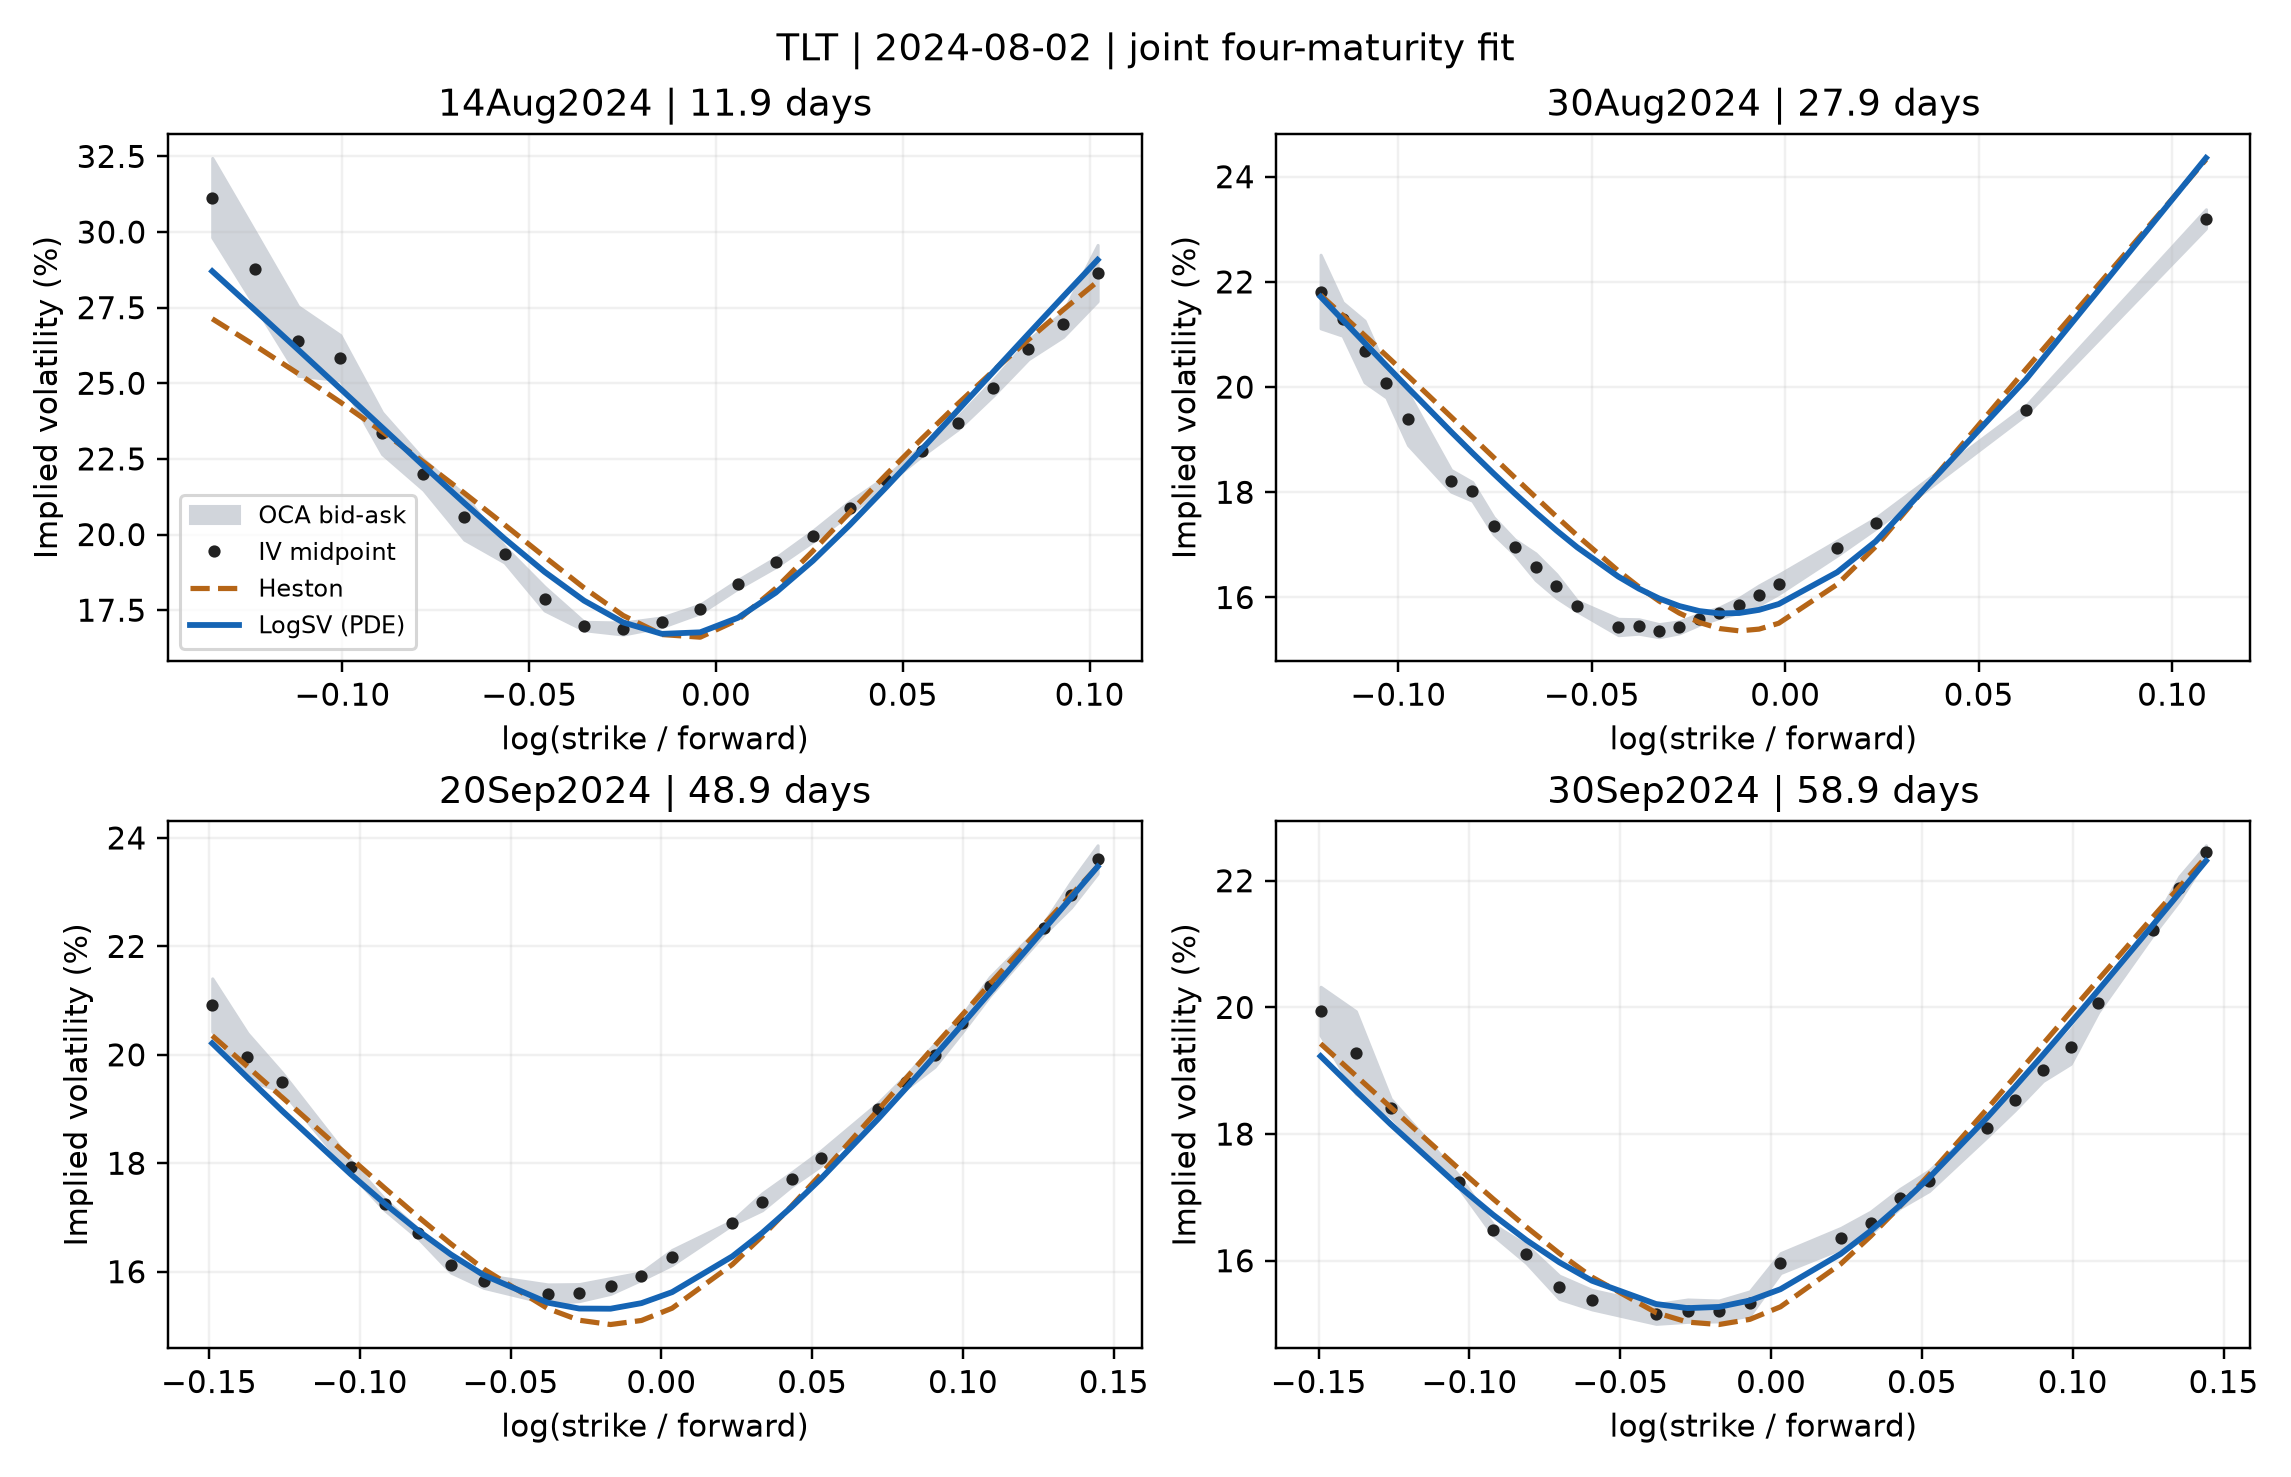
\includegraphics[width=\textwidth]{figures/calibration_positive_skew_20261031/tlt_fits.png}
\caption{TLT+ on 2 August 2024, including the approximately 12-day expiry. Points and grey bands show OCA midpoint and bid--ask IVs. The dashed curve is Heston and the solid curve the LogSV fit priced on the fine PDE grid. All four maturities share one parameter vector per model. The ETF panels use OCA European-equivalent Black IV conventions. Source: ThetaData via OCA.}\label{fig:oca-tltpositive}\end{figure}

% [AI-DRAFT BEGIN: per-maturity reading, information criterion and half-lives, 30 Oct 2026.]
Table~\ref{tab:oca-fits} summarises the four joint fits, and
Figures~\ref{fig:oca-spxw} and~\ref{fig:oca-tltpositive} show the SPXW and TLT+
smiles with both fitted curves. The GLD and July TLT smile figures are in the
replication package. Table~\ref{tab:oca-maturity} locates the improvement. On SPXW the LogSV RMSE at
the 12-day and 30-day slices is 0.66 and 0.46 percentage points against 1.13 and 0.62 for Heston, while the two longest slices differ by less. On GLD and TLT
the improvement is spread across maturities, and LogSV improves 15 of the 16 slices in total. A criterion of the Bayesian-information type
uses the unweighted per-quote sum $\mathrm{RSS}=\sum_{i,j}(100e_{ij})^2$,
evaluated at each model's fitted parameters, and $n=\sum_i n_i$, rather than the maturity-weighted objective in
\eqref{eq:oca-calibration-objective}. The statistic $n\ln(\mathrm{RSS}/n)+k\ln n$,
with $k=5$ for Heston and $k=6$ for LogSV, favours LogSV by SPXW: -88, GLD: -67, TLT: -76, TLT+: -56 (differences LogSV minus Heston, so negative values favour LogSV). The quotes
within a slice are not independent and some fitted parameters are at their bounds,
so the criterion is descriptive and the penalty
for the sixth parameter, $\ln n\approx4.6$, is small against the residual term.
The fitted parameters in Tables~\ref{tab:oca-logsv-params}
and~\ref{tab:oca-heston-params} carry linearised drift half-lives
$365\ln2/(\kappa_1+\kappa_2\theta)$ of 7.4 to 10.0 days for LogSV
and variance-mean half-lives $365\ln2/\kappa$ of 8.4 to 10.4 days for Heston, with active upper bounds on the drift speeds in
every LogSV fit and in the GLD and TLT+ Heston fits. Both models use their mean reversion to
shape the 12-day slice. The drift parameters are therefore term-structure parameters
of one snapshot, not estimates of historical mean reversion. The LogSV half-life
describes the drift linearised at $\theta$, rather than the exact conditional mean
or stationary autocorrelation. Heston's expression is exact for its conditional
variance mean.
% [AI-DRAFT END]

\begin{table}[htbp]\centering\small
\begin{tabular}{@{}l r r r r r r r r@{}}\toprule
Market & $\sigma_0$ & $\theta$ & $\kappa_1$ & $\kappa_2$ & $\beta$ & $\varepsilon$ & $\kappa_2-\beta$ & Half-life (days)\\\midrule

SPXW & 0.0722 & 0.1359 & 30.0000 & 1.5350 & -4.1765 & 4.7239 & 5.7115 & 8.4 \\

GLD & 0.1808 & 0.3021 & 1.2073 & 80.0000 & -1.2408 & 4.3198 & 81.2408 & 10.0 \\

TLT & 0.0758 & 0.0777 & 30.0000 & 13.6871 & -0.7883 & 5.7683 & 14.4754 & 8.1 \\

TLT+ & 0.1813 & 0.1280 & 30.0000 & 31.0183 & 1.4335 & 6.8799 & 29.5848 & 7.4 \\

\bottomrule\end{tabular}
\caption{PDE-calibrated LogSV parameters. The three July snapshots have $\beta<0$, and
TLT+ has $\beta>0$ and satisfies $\kappa_2>\beta$ with a wide margin. The imposed
lower bound $m=0.05$ is inactive for TLT+. Active bounds: SPXW $\kappa_1=30$, GLD $\kappa_2=80$, TLT $\kappa_1=30$, TLT+ $\kappa_1=30$. The linearised drift half-life is
$365\ln2/(\kappa_1+\kappa_2\theta)$. Source: ThetaData via OCA, with dates as in Table~\ref{tab:oca-fits}.}
\label{tab:oca-logsv-params}\end{table}

\begin{table}[htbp]\centering\small
\begin{tabular}{@{}l r r r r r r@{}}\toprule
Market & $V_0$ & $\theta_V$ & $\kappa$ & $\rho$ & $\nu$ & Half-life (days)\\\midrule

SPXW & 0.00353 & 0.03453 & 24.26049 & -0.64219 & 2.79164 & 10.4 \\

GLD & 0.04286 & 0.06558 & 30.00000 & -0.27978 & 2.77467 & 8.4 \\

TLT & 0.00585 & 0.01156 & 26.68251 & -0.13692 & 1.71334 & 9.5 \\

TLT+ & 0.04433 & 0.02625 & 30.00000 & 0.19569 & 3.11254 & 8.4 \\

\bottomrule\end{tabular}
\caption{Heston variance parameters. GLD and TLT+ reach the $\kappa=30$ upper bound. All
four solutions have $2\kappa\theta_V<\nu^2$, and the transform pricer accommodates
the attainable, instantaneously reflecting zero variance boundary of the usual CIR
solution. The conditional variance-mean half-life is $365\ln2/\kappa$. Source: ThetaData via OCA, with dates as in Table~\ref{tab:oca-fits}.}
\label{tab:oca-heston-params}\end{table}

\paragraph{Numerical checks.}
We separately double the spatial and the time resolution, enlarge the state domain
from six to eight log-volatility units at matched mesh spacing, and refine the
Fourier integration to 96 points per subinterval and cutoff 2400. Table~\ref{tab:oca-pde-checks}
reports the largest changes relative to the reported grid, in IV units and relative
to each quote's premium bid--ask spread, including the worst quote.

\begin{table}[htbp]\centering\small
\begin{tabular}{@{}l r r r r@{}}\toprule
Market & Grid IV change & Grid/spread & PDE--MC gap & MC steps\\
 & (pp, max.) & (\%, max.) & (bp of $F$, max.) & \\\midrule

SPXW & 0.00074 & 0.150 & 0.0187 & 512 \\

GLD & 0.00005 & 0.003 & 0.0067 & 1024 \\

TLT & 0.00014 & 0.021 & 0.0027 & 512 \\

TLT+ & 0.00027 & 0.057 & 0.0135 & 512 \\

\bottomrule\end{tabular}
\caption{All observed deterministic refinement changes are below one percent of a
premium spread at every retained quote, and independent Monte Carlo (MC) comparisons are
reported alongside them. Checks use the final PDE-calibrated parameters. Grid
columns take the maximum over four separate refinements. MC uses four independent
scrambles of 32768 paths each with paired half-step comparisons. Price differences
are discounted premiums divided by the forward, times $10^4$.}
\label{tab:oca-pde-checks}\end{table}

The largest deterministic refinement change is 0.00074 IV percentage
points and 0.150\% of a premium spread. Independent conditional
split-step Monte Carlo gives a maximum standardised price gap of 3.50, and 6 of the 393 quotes lie outside two
estimated scramble standard errors. Four scrambles give noisy standard-error
estimates, so these are not simultaneous tests. The simulator reports no volatility
flooring, and the Heston independent-pricing checks are retained in the replication package.

\paragraph{Cost, accuracy and what the examples support.}
% [AI-DRAFT BEGIN: speed and expansion status stated directly (E4), 30 Oct 2026.]
The PDE calibration costs 806 to 2,367 times the Heston transform calibration on these surfaces
(Table~\ref{tab:oca-fits}). These ratios compare the two implementations and their
starting protocols and do not isolate an intrinsic model cost. PDE fits include
two coarse starts and refinement, while simulation-based starting fits and validation
are excluded. A state-dependent PDE is solved at each Fourier frequency.
The second-order affine expansion of \citet{SeppRakhmonovLogSV} closes most of that
gap when it is accurate, but in the package's pricing diagnostics its truncation error is of
the same order as the smile residuals, and tighter solver tolerances, subdivision,
recentring and higher polynomial degree do not provide a general cure. We therefore
use the PDE for the objective and the displayed prices, reserve the expansion for
parameter regimes in which it has been validated against the PDE, and record the
regime boundary as an open implementation item.

The examples support limited conclusions. LogSV lowers the midpoint IV
RMSE on all four snapshots at one extra parameter, on 15 of 16 maturity
slices, with the largest gain at the 12-day SPXW slice. A numerically validated pricer does not make the model
fit each bid--ask interval, and the SPXW smile residuals remain material. The
implementation sequence that produced these numbers, a deterministic coarse-grid
fit, finer-grid refinement and independent checks at the final parameters judged
against market spreads, is the reusable part. The examples do not rank the model
families across assets and do not estimate historical mean reversion.

The TLT+ fit gives $\beta=\positiveBeta$ and $\kappa_2=\positiveKappaTwo$, hence
$\kappa_2-\beta=\positiveMargin$, and Heston gives $\rho=\positiveHestonRho$.
Its IV RMSE falls from \rmseHestonTLTpositive\ to \rmseLogSVTLTpositive\ percentage
points and its inside-spread share rises from \insideHestonTLTpositive\% to
\insideLogSVTLTpositive\%. The positive-dependence fit is admissible, with a slack
imposed constraint, and does not exercise $C=\beta$. Neither fitted coefficient is
the historical index beta of Section~\ref{sec:empirical-beta}. The ETF quotation
qualification applies.
% [AI-DRAFT END]



\FloatBarrier

\section{Practical model selection}
\label{sec:selection}

Begin with the contract, its quoting and settlement conventions, the pricing measure and the observable to be fitted. Then apply the relevant admissibility conditions before comparing fit quality and numerical cost. Table~\ref{tab:selection-guide} translates the preceding analysis into application-specific choices. It is a decision guide within the stated model domains, not a ranking that assigns a single winner to each asset class.

{\small
\setlength{\tabcolsep}{4pt}
\renewcommand{\arraystretch}{1.15}
\begin{longtable}{@{}P{31mm}P{56mm}P{58mm}@{}}
\caption{Practical model-selection guide. Mathematical restrictions refer to Sections~\ref{sec:framework}--\ref{sec:nonmarkov}, and observation and pricing checks refer to Sections~\ref{sec:observations} and~\ref{sec:oca-calibration}.}\label{tab:selection-guide}\\
\toprule
Application requirement & Model implication & Required check\\
\midrule
\endfirsthead
\multicolumn{3}{l}{\small Table~\thetable\ continued}\\
\toprule
Application requirement & Model implication & Required check\\
\midrule
\endhead
\bottomrule
\endfoot
European vanilla smile fitting & Use Heston as a parsimonious transform-pricing benchmark. Compare quadratic LogSV where its additional flexibility improves the target smiles by more than the quote width. The 3/2 model is a theoretical comparator here, and only its stationary marginal is compared in Table~\ref{tab:empirical-scores}. & Match quotes, forwards, discounts and objective weights. Report parameter counts, per-maturity residuals (Table~\ref{tab:oca-maturity}) and bid--ask agreement. Treat binding search bounds as a qualification of the fit.\\
\addlinespace
Positive instantaneous return--volatility dependence & Heston allows positive $\rho$ in its stated domain. Quadratic LogSV allows positive $\beta$ with $C\geq\beta$, and the 3/2 condition is $c-\rho\nu\geq-\nu^2/2$. Linear-drift LogSV does not support positive $\beta$ under the true-martingale requirement. & Apply conditions to the specified state dynamics. An index-regression coefficient or observed smile skew is not the latent $\beta$ or $\rho$. Check the observation map before interpreting a measured sign.\\
\addlinespace
Numeraire changes within the asset class & Derive the drift correction for the chosen numeraire (Table~\ref{tab:numeraires}). In quadratic LogSV, $C_S=C_Q-\beta$. In Heston, the stock-candidate mean-reversion coefficient becomes $\kappa-\rho\nu$. A quanto adjustment with deterministic exchange-rate volatility moves only the linear coefficient of quadratic LogSV and takes Heston outside its affine drift family. Under the annuity measure of a factor Heath--Jarrow--Morton model the quadratic coefficient becomes state dependent. & Validate the density on the required horizon and define the payoff and settlement currency. Family closure alone does not validate the measure. Stationarity under the new measure is a separate question.\\
\addlinespace
Historical persistence and long-run distributions & Specify stationarity under the measure used for the historical model. The Gamma, inverse-Gamma and GIG families imply different moment and tail restrictions. Stationary shape alone does not identify the volatility clock. & Distinguish implied-index dynamics from latent spot volatility, and match units and sampling conventions. Account for initialisation and finite-sample ACF effects before interpreting persistence or drift estimates.\\
\addlinespace
Short-maturity structure or explicit path dependence & Consider additional factors, Volterra or signature specifications when the target behaviour requires them. Use the model-specific criteria in Table~\ref{tab:nonmarkov}. Rough Bergomi and Volterra Heston have different martingality restrictions. & State the target option-implied statistic and horizon. Daily index ACF curvature alone does not identify latent roughness. Recheck pricing accuracy and admissibility for the chosen kernel or signature truncation.\\
\addlinespace
American ETF option applications & An exercise-aware engine or a validated European-equivalent conversion is needed for the intended use. The GLD and TLT examples here compare smiles under the European-equivalent convention of the data source. & Do not interpret these examples as exact American-option prices. Retain the forward, dividend and conversion assumptions. The effective parity discounts are not risk-free curve estimates.\\
\addlinespace
Reliable calibration across the fitted domain & For the tested Markovian, flat-backbone LogSV specification, use a deterministic full-state PDE fit followed by finer-grid refinement. A finite transform expansion is a fast approximation only within an independently validated regime. & Check the worst quote as well as aggregate error. Vary state, time, domain and Fourier resolution separately, then compare final prices with independent simulation. Express numerical error relative to quote spreads.\\
\end{longtable}
}

% [AI-DRAFT BEGIN: guide walk-through with macro numbers, 30 Oct 2026.]
The surface examples illustrate how to apply the guide. PDE-calibrated LogSV reduces the total IV RMSE from \rmseHestonSPXW{} to \rmseLogSVSPXW{} percentage points for SPXW, from \rmseHestonGLD{} to \rmseLogSVGLD{} for GLD, from \rmseHestonTLT{} to \rmseLogSVTLT{} for July TLT, and from \rmseHestonTLTpositive{} to \rmseLogSVTLTpositive{} for positive-skew TLT, and it improves \improvedSlices{} of \totalSlices{} maturity slices (Table~\ref{tab:oca-maturity}). The last case fits $\beta=\positiveBeta>0$ with $C-\beta=\positiveMargin$, so the imposed martingale margin is slack. Only \insideLogSVSPXW\% of the SPXW LogSV quotes lie inside their bid--ask intervals, and every LogSV fit has an active drift bound. The guide therefore asks for residual shape, active constraints and cost alongside the total score.

For implementation, accept a candidate only after its price accuracy is adequate for the intended quote tolerance, then decide whether its remaining fit improvement warrants the extra parameters and computational cost. On these surfaces the PDE calibration costs \fitRatioMin{} to \fitRatioMax{} times the Heston transform calibration. The ratio compares two implementations with different engines and starting procedures, and Section~\ref{sec:oca-calibration} states what would close the gap. A more elaborate model is useful when it addresses a specified residual or dynamic requirement that matters for the application.
% [AI-DRAFT END]

\section{Discussion}
\label{sec:discussion}

% [AI-DRAFT BEGIN: discussion rewritten around the closure rule, the evidence and the open items, 30 Oct 2026.]
A robust stochastic-volatility model, in the sense of this paper, is one whose drift family contains the corrections of its numeraire and measure changes and whose corrected coefficients satisfy the validity and martingale thresholds on the horizons of the application. Proposition~\ref{prop:closure} makes the first part a one-exponent test whenever a correction is nonzero. Proposition~\ref{prop:affine-closure} adds deterministic kernels, and among the seven diffusion specifications only signed Gaussian volatility and quadratic-drift lognormal volatility are closed under both kernel types. Sections~\ref{sec:diffusions} and~\ref{sec:quadratic} supply the thresholds: all \(\rho\) for Heston, \(c-\rho\nu\geq-\nu^2/2\) for the 3/2 model and \(C\geq\beta\) for quadratic-drift lognormal volatility, with \(\rho\leq0\) or \(\beta\leq0\) for the exponential-OU, GARCH-diffusion and linear-drift lognormal families whose nonzero corrections leave the specified drift family. Measure validity, volatility regularity, stationarity and numerical reliability remain separate requirements, and the non-Markovian results of Section~\ref{sec:nonmarkov} hold under their own published hypotheses.

The index evidence informs observed dependence and marginal fit, with implications for latent dynamics conditional on the observation map of Section~\ref{sec:observations}. Positive observed slopes occur on \betaPosGVZ\% of GVZ days, \betaPosVXTLT\% of VXTLT days, \betaPosMOVE\% of MOVE days, and \betaPosBTCDVOL\% and \betaPosETHDVOL\% of BTC and ETH DVOL days, which motivates models capable of reproducing positive observed dependence. Inferring a latent leverage sign from these daily slopes requires a specified observation model. The held-out marginal comparison favours the GIG family over the Heston marginal for \panelGigWins{} of \panelCount{} Cboe indices, cannot separate the two power-tailed laws on VIX and BTC DVOL, and favours the 3/2 marginal on ETH DVOL, so no single stationary family transfers best across assets. The VIX and OVX index marginals select the inverse-Gamma boundary within the fitted family. These index fits motivate considering \(C_P=0\) as a latent-model hypothesis, but do not establish that hypothesis or locate a quadratic term in one measure. The separate mathematical argument is that positive latent \(\beta\) requires \(C_Q\geq\beta\), and a latent physical model with \(C_P=0\) can satisfy this through \(\beta\ell_0+\varepsilon\ell_1\geq\max(\beta,0)\).

The option-surface calibrations connect the framework to implementation. LogSV lowers the in-sample IV RMSE on all four snapshots and on \improvedSlices{} of \totalSlices{} maturity slices at one additional parameter, with active drift bounds and linearised-drift half-lives of \halfLifeLogSVMin{} to \halfLifeLogSVMax{} days that describe the term structure of the snapshots. The positive-skew TLT snapshot is fitted with \(\beta=\positiveBeta\) and \(C-\beta=\positiveMargin\), so the imposed admissibility constraint is slack and the boundary is not tested. The ETF results remain conditional on the European-equivalent quotation convention. The PDE calibration costs \fitRatioMin{} to \fitRatioMax{} times the Heston transform calibration under the reported implementations, and the second-order expansion that would remove most of that cost is reliable only inside a regime that remains to be delimited. Two items are open: the validated regime of the expansion, and joint inference of latent dynamics from realised and implied volatility.
% [AI-DRAFT END]

\appendix
\section{Boundary proof for quadratic-drift volatility}
\label{app:proof}

\subsection{Positive solutions and explosion at infinity}

Consider, up to its lifetime, the auxiliary scalar diffusion
\begin{equation}
 \dd X_t=(A+BX_t-DX_t^2)\dd t+vX_t\dd W_t,\qquad
 X_0>0,\quad A\geq0,\quad v>0.
 \label{eq:auxiliary}
\end{equation}
The coefficients are locally Lipschitz on \((0,\infty)\). Zero cannot be reached in finite time. Indeed, on \(0<X_t\leq1\), the logarithmic drift satisfies
\[
 \frac{A}{X_t}+B-DX_t-\frac{v^2}{2}
 \geq B-\max(D,0)-\frac{v^2}{2}.
\]
A localised logarithmic argument, using boundedness of a Brownian path on a compact time interval, excludes convergence to minus infinity at a finite lower-boundary hitting time. This also covers \(A=0\).

Write \(\eta=2B/v^2-1\), as in Section~\ref{sec:quadratic}. Up to a positive multiplicative constant, the scale and speed densities are
\begin{equation}
 s_D'(x)=x^{-\eta-1}\exp\left(\frac{2A}{v^2x}+\frac{2Dx}{v^2}\right),
 \qquad
 m_D(x)=\frac{2}{v^2x^2s_D'(x)}.
 \label{eq:scale-speed}
\end{equation}
If \(D>0\), the scale function satisfies \(s_D(\infty)=\infty\), so infinity is inaccessible. If \(D=0\), the same holds when \(\eta\leq0\). When \(D=0,\eta>0\),
\[
 [s_D(\infty)-s_D(x)]m_D(x)
 \sim\frac{2}{v^2\eta x},\qquad x\to\infty.
\]
The integral diverges, so Feller's boundary test again excludes explosion. Therefore \(D\geq0\) gives a unique positive global strong solution. Applying this with \(D=C\) proves the regularity assertion in Proposition~\ref{prop:martingale}.

If \(D<0\), then \(s_D(\infty)<\infty\) and
\[
 [s_D(\infty)-s_D(x)]m_D(x)
 \sim\frac{1}{(-D)x^2},\qquad x\to\infty.
\]
Its finite integral makes infinity accessible.

Explosion has positive probability before every \(T>0\). To see the time-horizon statement directly, put \(d=-D>0\) and \(Y=1/X\). Until \(Y\) reaches zero,
\[
 \dd Y_t=[-d+(v^2-B)Y_t-AY_t^2]\dd t-vY_t\dd W_t.
\]
By one-dimensional comparison, \(Y\) is bounded above, up to the relevant zero hitting times, by
\[
 \dd U_t=[-d+(v^2-B)U_t]\dd t-vU_t\dd W_t,\qquad U_0=Y_0.
\]
With \(H_t=\exp((v^2/2-B)t-vW_t)\), the latter solution is
\[
 U_t=H_t\left(Y_0-d\int_0^tH_u^{-1}\dd u\right).
\]
Brownian motion has full support on continuous paths over \([0,T]\), so the integral \(\int_0^TH_u^{-1}\dd u\) has unbounded support for every \(T>0\). Thus \(U\), and hence \(Y\), reaches zero before \(T\) with positive probability.

\subsection{Stopped densities and loss of mass}

% [AI-DRAFT BEGIN: difficulty signpost (M1), 30 Oct 2026.]
The step that needs care is the passage from the boundary classification above to a statement about \(\E^Q[S_T]\). The stock-numeraire measure cannot be assumed, because its existence is what is being decided, so the density is stopped at the volatility level \(n\), where Novikov's condition holds, and the global statement is recovered as a limit in \(n\) through the explosion time of the auxiliary diffusion.
% [AI-DRAFT END]

Set \(M_t=S_t/S_0\) and \(\tau_n=\inf\{t:\sigma_t\geq n\}\), with \(n>\sigma_0\). The stopped exponential \(M_{t\wedge\tau_n}\) is a true martingale by Novikov's condition. Under its finite-horizon density, stopped volatility has drift
\[
 A+B\sigma-(C-\beta)\sigma^2.
\]
Uniqueness in law up to exit identifies these stopped dynamics with the auxiliary diffusion~\eqref{eq:auxiliary} for \(D=C-\beta\).

Let \(\widetilde{\PP}\) denote the law of that auxiliary diffusion, \(\widetilde\tau_n\) its upper hitting times, and \(\zeta\) its explosion time. Nonexplosion of the original volatility and monotone convergence yield
\begin{align*}
 \E^Q[M_T]
 &=\lim_{n\to\infty}\E^Q[M_T\ind_{\{\tau_n>T\}}]\\
 &=\lim_{n\to\infty}\widetilde{\PP}(\widetilde\tau_n>T)
 =\widetilde{\PP}(\zeta>T).
\end{align*}
No global stock-numeraire measure has been assumed in this argument. The boundary calculation shows that the last probability is one for every finite \(T\) exactly when \(C-\beta\geq0\). A nonnegative local martingale with constant expectations is a true martingale. If \(C-\beta<0\), the positive explosion probability established above gives the strict expectation defect for every \(T>0\).

\FloatBarrier

\begin{thebibliography}{99}

\bibitem[Abi Jaber et~al.(2025)]{AbiJaberGassiatSotnikov2025}
Abi Jaber, E., Gassiat, P. and Sotnikov, D. (2025).
Martingale property and moment explosions in signature volatility models.
Preprint, version 2, \url{https://arxiv.org/abs/2503.17103v2}.

\bibitem[Abi Jaber et~al.(2019)]{AbiJaberLarssonPulido2019}
Abi Jaber, E., Larsson, M. and Pulido, S. (2019).
Affine Volterra processes.
\emph{Annals of Applied Probability}, 29(5), 3155--3200.
\href{https://doi.org/10.1214/19-AAP1477}{doi:10.1214/19-AAP1477}.

\bibitem[Abi Jaber and Li(2025)]{AbiJaberLi2025}
Abi Jaber, E. and Li, S.~X. (2025).
Volatility models in practice: Rough, path-dependent, or Markovian?
\emph{Mathematical Finance}, 35(4), 796--817.
\href{https://doi.org/10.1111/mafi.12463}{doi:10.1111/mafi.12463}.

\bibitem[Abi Jaber and Sotnikov(2025)]{AbiJaberSotnikov2025}
Abi Jaber, E. and Sotnikov, D. (2025).
Exponentially fading memory signature.
Preprint, version 2, \url{https://arxiv.org/abs/2507.03700v2}.

\bibitem[Andersen and Piterbarg(2007)]{AndersenPiterbarg2007}
Andersen, L.~B.~G. and Piterbarg, V.~V. (2007).
Moment explosions in stochastic volatility models.
\emph{Finance and Stochastics}, 11, 29--50.
\href{https://doi.org/10.1007/s00780-006-0011-7}{doi:10.1007/s00780-006-0011-7}.

\bibitem[Baldeaux and Badran(2014)]{BaldeauxBadran2014}
Baldeaux, J. and Badran, A. (2014).
Consistent modelling of VIX and equity derivatives using a 3/2 plus jumps model.
\emph{Applied Mathematical Finance}, 21(4), 299--312.
\href{https://doi.org/10.1080/1350486X.2013.868631}{doi:10.1080/1350486X.2013.868631}.

\bibitem[Bayer et~al.(2016)]{BayerFrizGatheral2016}
Bayer, C., Friz, P. and Gatheral, J. (2016).
Pricing under rough volatility.
\emph{Quantitative Finance}, 16(6), 887--904.
\href{https://doi.org/10.1080/14697688.2015.1099717}{doi:10.1080/14697688.2015.1099717}.

\bibitem[Bennedsen et~al.(2022)]{BennedsenLundePakkanen2022}
Bennedsen, M., Lunde, A. and Pakkanen, M.~S. (2022).
Decoupling the short- and long-term behavior of stochastic volatility.
\emph{Journal of Financial Econometrics}, 20(5), 961--1006.
\href{https://doi.org/10.1093/jjfinec/nbaa049}{doi:10.1093/jjfinec/nbaa049}.

\bibitem[Bergomi(2005)]{Bergomi2005}
Bergomi, L. (2005).
Smile dynamics II.
\emph{Risk}, October 2005, 67--73.

\bibitem[Bergomi(2016)]{Bergomi2016}
Bergomi, L. (2016).
\emph{Stochastic Volatility Modeling}.
Chapman and Hall/CRC, Boca Raton.

\bibitem[Bergomi and Guyon(2012)]{BergomiGuyon2012}
Bergomi, L. and Guyon, J. (2012).
Stochastic volatility's orderly smiles.
\emph{Risk}, May 2012, 60--66.

\bibitem[Bernard et~al.(2017)]{BernardCuiMcLeish2017}
Bernard, C., Cui, Z. and McLeish, D. (2017).
On the martingale property in stochastic volatility models based on time-homogeneous diffusions.
\emph{Mathematical Finance}, 27(1), 194--223.
\href{https://doi.org/10.1111/mafi.12084}{doi:10.1111/mafi.12084}.

\bibitem[Carr and Sun(2007)]{CarrSun2007}
Carr, P. and Sun, J. (2007).
A new approach for option pricing under stochastic volatility.
\emph{Review of Derivatives Research}, 10(2), 87--150.
\href{https://doi.org/10.1007/s11147-007-9014-6}{doi:10.1007/s11147-007-9014-6}.

\bibitem[Carr and Willems(2019)]{CarrWillems2019}
Carr, P. and Willems, S. (2019).
A lognormal type stochastic volatility model with quadratic drift.
Preprint, version 1, \url{https://arxiv.org/abs/1908.07417v1}.

\bibitem[Cheridito et~al.(2003)]{CheriditoKawaguchiMaejima2003}
Cheridito, P., Kawaguchi, H. and Maejima, M. (2003).
Fractional Ornstein--Uhlenbeck processes.
\emph{Electronic Journal of Probability}, 8, paper 3, 1--14.
\href{https://doi.org/10.1214/EJP.v8-125}{doi:10.1214/EJP.v8-125}.

\bibitem[Christoffersen et~al.(2010)]{ChristoffersenJacobsMimouni2010}
Christoffersen, P., Jacobs, K. and Mimouni, K. (2010).
Volatility dynamics for the S\&P500: Evidence from realized volatility, daily returns, and option prices.
\emph{Review of Financial Studies}, 23(8), 3141--3189.
\href{https://doi.org/10.1093/rfs/hhq032}{doi:10.1093/rfs/hhq032}.

\bibitem[Cont and Das(2024)]{ContDas2024}
Cont, R. and Das, P. (2024).
Rough volatility: Fact or artefact?
\emph{Sankhya B}, 86(1), 191--223.
\href{https://doi.org/10.1007/s13571-024-00322-2}{doi:10.1007/s13571-024-00322-2}.

\bibitem[Cox and Hobson(2005)]{CoxHobson2005}
Cox, A.~M.~G. and Hobson, D.~G. (2005).
Local martingales, bubbles and option prices.
\emph{Finance and Stochastics}, 9(4), 477--492.
\href{https://doi.org/10.1007/s00780-005-0162-y}{doi:10.1007/s00780-005-0162-y}.

\bibitem[Cuchiero et~al.(2023)]{CuchieroGazzaniSvalutoFerro2023}
Cuchiero, C., Gazzani, G. and Svaluto-Ferro, S. (2023).
Signature-based models: Theory and calibration.
\emph{SIAM Journal on Financial Mathematics}, 14(3), 910--957.
\href{https://doi.org/10.1137/22M1512338}{doi:10.1137/22M1512338}.

\bibitem[El Euch and Rosenbaum(2019)]{ElEuchRosenbaum2019}
El Euch, O. and Rosenbaum, M. (2019).
The characteristic function of rough Heston models.
\emph{Mathematical Finance}, 29(1), 3--38.
\href{https://doi.org/10.1111/mafi.12173}{doi:10.1111/mafi.12173}.

\bibitem[Friz and Gatheral(2025)]{FrizGatheral2025}
Friz, P.~K. and Gatheral, J. (2025).
Computing the SSR.
\emph{Quantitative Finance}, 25(5), 701--710.
\href{https://doi.org/10.1080/14697688.2025.2486173}{doi:10.1080/14697688.2025.2486173}.

\bibitem[Fukasawa(2026)]{Fukasawa2026}
Fukasawa, M. (2026).
On the skew stickiness ratio.
Preprint, version 2, \url{https://arxiv.org/abs/2602.05241v2}.

\bibitem[Gassiat(2019)]{Gassiat2019}
Gassiat, P. (2019).
On the martingale property in the rough Bergomi model.
\emph{Electronic Communications in Probability}, 24, paper 33, 1--9.
\url{https://arxiv.org/abs/1811.10935}.

\bibitem[Gatheral et~al.(2018)]{GatheralJaissonRosenbaum2018}
Gatheral, J., Jaisson, T. and Rosenbaum, M. (2018).
Volatility is rough.
\emph{Quantitative Finance}, 18(6), 933--949.
\href{https://doi.org/10.1080/14697688.2017.1393551}{doi:10.1080/14697688.2017.1393551}.

\bibitem[Guyon et~al.(2026)]{GuyonJeanninJourdain2026}
Guyon, J., Jeannin, T. and Jourdain, B. (2026).
The martingale property in Volterra volatility models.
Preprint, version 1, \url{https://arxiv.org/abs/2610.32684v1}.

\bibitem[Guyon and Lekeufack(2023)]{GuyonLekeufack2023}
Guyon, J. and Lekeufack, J. (2023).
Volatility is (mostly) path-dependent.
\emph{Quantitative Finance}, 23(9), 1221--1258.
\href{https://doi.org/10.1080/14697688.2023.2221281}{doi:10.1080/14697688.2023.2221281}.

\bibitem[Hagan et~al.(2002)]{HaganEtAl2002}
Hagan, P.~S., Kumar, D., Lesniewski, A.~S. and Woodward, D.~E. (2002).
Managing smile risk.
\emph{Wilmott Magazine}, September 2002, 84--108.

\bibitem[Hansen et~al.(1998)]{HansenScheinkmanTouzi1998}
Hansen, L.~P., Scheinkman, J.~A. and Touzi, N. (1998).
Spectral methods for identifying scalar diffusions.
\emph{Journal of Econometrics}, 86(1), 1--32.
\href{https://doi.org/10.1016/S0304-4076(97)00107-3}{doi:10.1016/S0304-4076(97)00107-3}.

\bibitem[Heston(1993)]{Heston1993}
Heston, S.~L. (1993).
A closed-form solution for options with stochastic volatility with applications to bond and currency options.
\emph{Review of Financial Studies}, 6(2), 327--343.
\href{https://doi.org/10.1093/rfs/6.2.327}{doi:10.1093/rfs/6.2.327}.

\bibitem[Jourdain(2004)]{Jourdain2004}
Jourdain, B. (2004).
Loss of martingality in asset price models with lognormal stochastic volatility.
Rapport de recherche CERMICS 2004-267, \'Ecole des Ponts ParisTech.
\url{https://cermics.enpc.fr/cermics-rapports-recherche/2004/CERMICS-2004/CERMICS-2004-267.pdf}.

\bibitem[Karasinski and Sepp(2012)]{KarasinskiSepp2012}
Karasinski, P. and Sepp, A. (2012).
Beta stochastic volatility model.
\emph{Risk}, October 2012, 66--71.
% [AUTHOR: pages 66--71 follow your IJTAF 2023 and RDR 2025 reference lists, your 2012 slides and the SSRN record.
%  The ZBW/EconBiz catalogue entry of the journal issue lists pages 62--68. Check against the print issue.]

\bibitem[Lewis(2000)]{Lewis2000}
Lewis, A.~L. (2000).
\emph{Option Valuation under Stochastic Volatility}.
Finance Press, Newport Beach.

\bibitem[Lions and Musiela(2007)]{LionsMusiela2007}
Lions, P.-L. and Musiela, M. (2007).
Correlations and bounds for stochastic volatility models.
\emph{Annales de l'Institut Henri Poincar\'e C, Analyse non lin\'eaire},
24(1), 1--16.
\href{https://doi.org/10.1016/j.anihpc.2005.05.007}{doi:10.1016/j.anihpc.2005.05.007}.

\bibitem[Lipton and Sepp(2008)]{LiptonSepp2008}
Lipton, A. and Sepp, A. (2008).
Stochastic volatility models and Kelvin waves.
\emph{Journal of Physics A: Mathematical and Theoretical}, 41(34), 344012.
\href{https://doi.org/10.1088/1751-8113/41/34/344012}{doi:10.1088/1751-8113/41/34/344012}.

\bibitem[Lucic and Sepp(2024)]{LucicSepp2024}
Lucic, V. and Sepp, A. (2024).
Valuation and hedging of cryptocurrency inverse options.
\emph{Quantitative Finance}, 24(7), 851--869.
\href{https://doi.org/10.1080/14697688.2024.2364804}{doi:10.1080/14697688.2024.2364804}.

\bibitem[Mijatovi\'c and Urusov(2012)]{MijatovicUrusov2012}
Mijatovi\'c, A. and Urusov, M. (2012).
On the martingale property of certain local martingales.
\emph{Probability Theory and Related Fields}, 152, 1--30.
\href{https://doi.org/10.1007/s00440-010-0314-7}{doi:10.1007/s00440-010-0314-7}.

\bibitem[Posp\'{\i}\v{s}il et~al.(2019)]{PospisilSobotkaZiegler2019}
Posp\'{\i}\v{s}il, J., Sobotka, T. and Ziegler, P. (2019).
Robustness and sensitivity analyses for stochastic volatility models under uncertain data structure.
\emph{Empirical Economics}, 57(6), 1935--1958.
\href{https://doi.org/10.1007/s00181-018-1535-3}{doi:10.1007/s00181-018-1535-3}.

\bibitem[Sch\"obel and Zhu(1999)]{SchobelZhu1999}
Sch\"obel, R. and Zhu, J. (1999).
Stochastic volatility with an Ornstein--Uhlenbeck process: An extension.
\emph{European Finance Review}, 3(1), 23--46.
\href{https://doi.org/10.1023/A:1009803506170}{doi:10.1023/A:1009803506170}.

\bibitem[Sepp(2011)]{Sepp2011}
Sepp, A. (2011).
Efficient numerical PDE methods to solve calibration and pricing problems in local stochastic volatility models.
Presentation at Global Derivatives Trading and Risk Management, Paris, 12--15 April 2011.
{\def\UrlBreaks{\do\/\do\-}\url{https://www.slideshare.net/slideshow/efficient-numerical-pde-methods-to-solve-calibration-and-pricing-problems-in-local-stochastic-volatility-models/38509675}}. % hyphen breaks are allowed for this address only

\bibitem[Sepp and Rakhmonov(2023)]{SeppRakhmonovLogSV}
Sepp, A. and Rakhmonov, P. (2023).
Log-normal stochastic volatility model with quadratic drift.
\emph{International Journal of Theoretical and Applied Finance},
26(8), 2450003.
\href{https://doi.org/10.1142/S0219024924500031}{doi:10.1142/S0219024924500031}.

\bibitem[Sepp and Rakhmonov(2025)]{SeppRakhmonovFHJM2025}
Sepp, A. and Rakhmonov, P. (2025).
Stochastic volatility for factor Heath--Jarrow--Morton framework.
\emph{Review of Derivatives Research}, 28(3). % [AUTHOR: the article number was not found in the sources checked. The DOI identifies the paper.]
\href{https://doi.org/10.1007/s11147-025-09217-4}{doi:10.1007/s11147-025-09217-4}.

\bibitem[Sepp and Rakhmonov(2026)]{SeppRakhmonovRoughLogSV2026}
Sepp, A. and Rakhmonov, P. (2026).
Rough log-normal stochastic volatility with quadratic drift: Second-moment stability and the martingale property under positive correlation.
Working paper, revision 2 of 17 November 2026. % [AUTHOR: title as in the r2 source. Add the SSRN or arXiv identifier once posted.]

\bibitem[Sin(1998)]{Sin1998}
Sin, C.~A. (1998).
Complications with stochastic volatility models.
\emph{Advances in Applied Probability}, 30(1), 256--268.
\href{https://doi.org/10.1239/aap/1035228003}{doi:10.1239/aap/1035228003}.

\bibitem[Sotnikov and Viot(2026)]{SotnikovViot2026}
Sotnikov, D. and Viot, A. (2026).
Martingality in EFM signature volatility models.
Preprint, version 1, \url{https://arxiv.org/abs/2610.35022v1}.

\bibitem[Stein and Stein(1991)]{SteinStein1991}
Stein, E.~M. and Stein, J.~C. (1991).
Stock price distributions with stochastic volatility: An analytic approach.
\emph{Review of Financial Studies}, 4(4), 727--752.
\href{https://doi.org/10.1093/rfs/4.4.727}{doi:10.1093/rfs/4.4.727}.

\bibitem[Wong and Heyde(2006)]{WongHeyde2006}
Wong, B. and Heyde, C.~C. (2006).
On changes of measure in stochastic volatility models.
\emph{Journal of Applied Mathematics and Stochastic Analysis}, 2006, article 18130, 1--13.
\href{https://doi.org/10.1155/JAMSA/2006/18130}{doi:10.1155/JAMSA/2006/18130}.

\end{thebibliography}
\end{document}
